
\documentclass[11pt,twoside,a4paper]{book}

\newcommand{\sphere}{\mathds{S}^{d-1}}
\newcommand{\orto}{\mathds{O}^d}
\newcommand{\R}{\mathds{R}^d}
\newcommand{\spharm}{\mathds{Y}^d_n}
\newcommand{\sphint}{\int_{\sphere}}
\usepackage[spanish,activeacute]{babel} % Para poner acentos y ñ en español
\usepackage[T1]{fontenc}
\usepackage[utf8]{inputenc}
\usepackage{lmodern}
\usepackage{amsmath}
\usepackage{amsthm}
\usepackage{amssymb}
\usepackage{latexsym}
\usepackage{graphicx}
\usepackage[hidelinks=true]{hyperref}
\usepackage{dsfont}
\usepackage{appendix}
\usepackage{graphicx}
\usepackage{float}
%Numeracion de teoremas, proposiciones, etc.
\numberwithin{equation}{section}
\numberwithin{figure}{section}
\theoremstyle{plain}
\newtheorem{thm}{Teorema}[chapter]
  \theoremstyle{definition}
        \newtheorem{defn}[thm]{Definici\'{o}n}
        \theoremstyle{plain}
  \newtheorem{prop}[thm]{Proposici\'{o}n}
        \theoremstyle{definition}
        \newtheorem{example}[thm]{Ejemplo}
  \theoremstyle{remark}
        \newtheorem{rem}[thm]{Nota}
  \theoremstyle{definition}
        \newtheorem{problem}[thm]{Problema}
  \theoremstyle{lem}
	  \newtheorem{lem}[thm]{Lema}
  \theoremstyle{cor}
  \newtheorem{cor}[thm]{Corolario}

\setlength{\oddsidemargin}{2cm}
\setlength{\evensidemargin}{1cm}

\DeclareGraphicsExtensions{.jpg,.pdf,.mps,.png}

\pagestyle{empty}

\begin{document}


\thispagestyle{empty}

%Portada

\begin{center}

%{\Large UNIVERSIDAD DE GRANADA}\\[8mm]
%{\Large Facultad de Ciencias}\\[8mm]
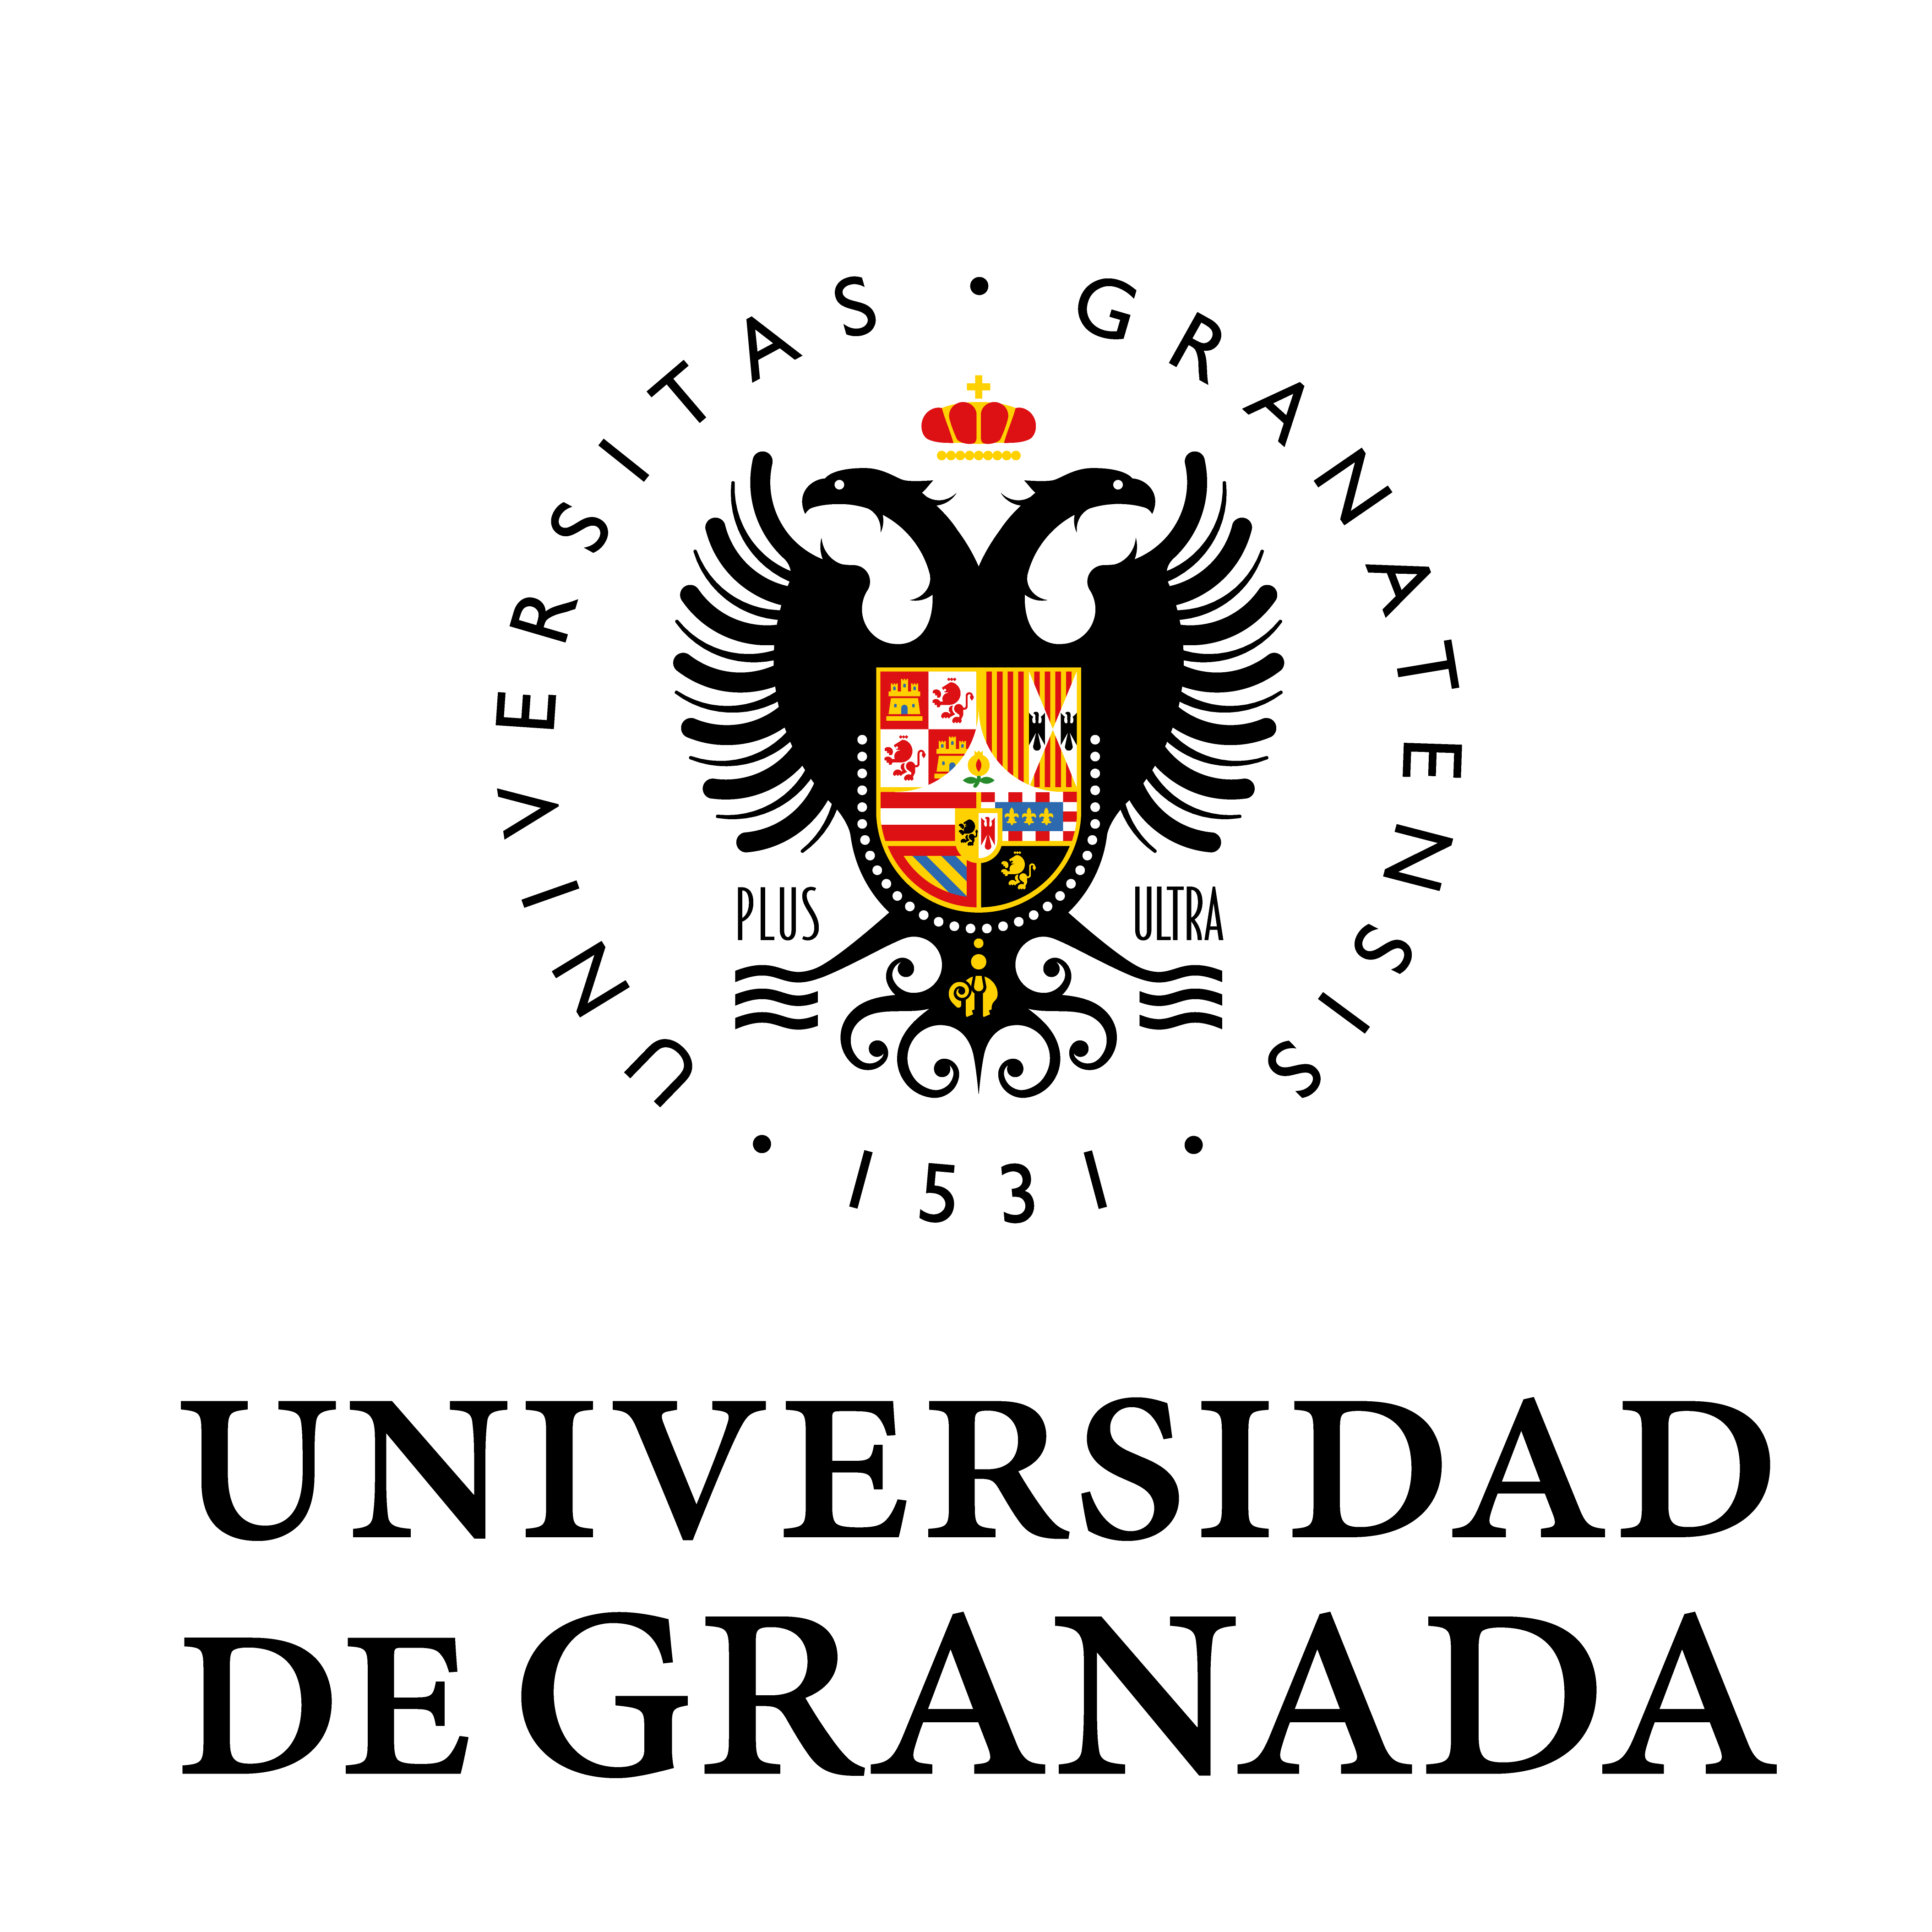
\includegraphics[width=9cm]{simbolo_color.png}\\[2cm]
{\Large\sffamily M\'aster Universitario en F\'isica y Matem\'aticas}\\[3mm]


\vspace{2cm}


\begin{Large}
{\slshape\bfseries  EL T\'ITULO DEL TRABAJO\\[6mm]
FIN DE M\'ASTER}
\end{Large}

\vspace{2cm}

\vfill

\begin{large}
{\bf Trabajo Fin de M\'aster presentado por \\[3mm]
Nombre Apellido1 Apellido2}
\end{large}


\vspace{1.5cm}

\begin{Large}
Curso 2016/17
\end{Large}
\end{center}




%%%%%%%%%%%%%%%%%%%%%%%%% Página en blanco, revés de la primera página

\quad

\thispagestyle{empty}


\newpage 

%%%%%%%%%%%%%%% Página de portada


\thispagestyle{empty}


\begin{center}

{\Large UNIVERSIDAD DE GRANADA}\\[10mm]
%{\Large Facultad de Ciencias}\\[4mm]
%\includegraphics[width=4cm]{escudo_ugr}\\[4mm]
{\Large\sffamily M\'aster Universitario en F\'isica y Matem\'aticas}\\[3mm]


\vspace{3cm}


\begin{Large}
{\slshape\bfseries  EL T\'ITULO DEL TRABAJO\\[6mm]
FIN DE M\'ASTER}
\end{Large}

\vspace{3cm}

\vfill

\begin{large}
{\bf Trabajo Fin de M\'aster presentado por \\[3mm]
Nombre Apellido1 Apellido2}
\end{large}


\vspace{2cm}

\begin{Large}
Curso 2016/17
\end{Large}
\end{center}

\vfill

\noindent
Tutor: Nombre Apellido1 Apellido2

\noindent
Departamento: Matem\'atica Aplicada

\noindent
\'Area de Conocimiento: Matem\'atica Aplicada

\newpage

%%%%%%%%%%%% Página en blanco, revés

\thispagestyle{empty}

\quad

\newpage

\thispagestyle{empty}

\vspace*{2cm}

\begin{flushright}
\parbox{3.5in}
{\small
(P\'agina de agradecimientos si los hay)


Thank you.}

\end{flushright}

\newpage




\newpage
\phantom{o}
\newpage

\pagenumbering{roman}
\setcounter{page}{3}

\renewcommand{\contentsname}{Índice}
\tableofcontents

\newpage
\phantom{o}
\newpage

\pagestyle{headings}

\setcounter{page}{1}
\pagenumbering{arabic}

%Si quieres poner tus propias marcas en el borde superior de las páginas
%\pagestyle{myheadings}
%\def\leftmark{\textsc{Nombre del autor}}
%\def\rightmark{\textsc{Trabajo Fin de Grado}}

%Cuerpo del trabajo, se incluye por cap´itulos

%\chapter*{Introducción}
\subsection*{Summary}

In this work, we consider systems of points on the unit sphere related to problems of approximation and numerical integration. This sistems are useful in various fields ranging from global climate models for the Earth, mapping of the stationary and magnetic fields of the Earth, crystallography, geodesic domes, virus modeling, computational geometry, etc.
\medskip

Starting with the construction of the spherical armonic space. Next, we study the Addition Theorem and its consequences. This result will allow us to generate an	 orthonormal basis of the space of spherical harmonics. 
Later, we get an expression for critical points of the gradient of a sherical armonic. In particular, we get critical points of the 3-dimensional sphere. 

Finally, we get some results about numeric quadrature.

\medskip
In the second part of the work, we explain the process followed for participation in a data mining competition. This process consists of the parts related to the understanding of the problem, the visualization of the data with which we will work, the application of preprocessing techniques to improve the data set and the choice of the algorithm to use to build a data model . Finally, we discuss the results obtained.

\bigskip
\emph{keywords:} sphere, spherical armonic, gradient, preprocessing, machine learning.
\newpage
\subsection*{Resumen}
Uno de los propósitos de este trabajo es determinar conjuntos de puntos para aproximación, interpolación e integración sobre la esfera y sus propiedades geométricas. Las distribuciones de puntos en la esfera unidad tienen aplicaciones que van desde modelos climáticos globales para la  Tierra, mapeado de los campos estacionales y magnéticos de la Tierra, cristalografía, cúpulas geodésicas, modelado de virus, geometría computacional, etc.

\medskip
Para ello, en primer lugar, introduciremos de forma constructiva el espacio de los armónicos esféricos sobre el que trabajaremos. Una vez construido dicho espacio, trataremos el Teorema de adición y sus consecuencias. Estos ingredientes nos permitirán generar una base ortonormal del espacio de esféricos armónicos.

Una vez asentadas las bases, estudiaremos el gradiente de dichos polinomios y calcularemos sus puntos críticos. Como caso particular, estudiaremos los puntos críticos de dichos polinomios sobre la esfera de dimensión tres y obtendremos una visualización de los resultados obtenidos.

Finalmente, trataremos varios resultados sobre integración numérica.
\bigskip

En la segunda parte del trabajo, explicaremos el proceso seguido durante la participación en una competición de data mining. Dicho proceso consta de las partes relativas a la comprensión del problema, la visualización de los datos con los que vamos a trabajar, la aplicación de técnicas de preprocesamiento para mejorar el conjunto de datos y la elección del algoritmo a usar para construir un modelo de datos. Finalmente, estudiaremos los resultados obtenidos y realizaremos un análisis sobre los mismos. 
	
\bigskip
\emph{Palabras clave:} esfera, armónicos, gradiente, preprocesamiento, clasificación.
\newpage


\subsection*{Objetivos.}
Los objetivos propuestos al inicio del trabajo fueron los siguientes:
\begin{itemize}
	\item Simulación y visualización de distribuciones de puntos sobre la esfera
	\item Estimación numérica de la calidad de las aproximaciones obtenidas mediante estas distribuciones de puntos. 
	\item Enfrentarse a un problema real de machine learning, estudiando las posibles soluciones y los resultados obtenidos.
\end{itemize}

El primer objetivo se ha logrado satisfactoriamente, siendo desarrollado en el Capítulo 2. El segundo objetivo se ha alcanzado durante el desarollo del Capítulo 3. Finalmente, el tercer objetivo se ha cumplido, siendo desarrollado en la segunda parte del trabajo.

\subsection*{Organización de la memoria.}
\medskip

El Capítulo 1 contiene todo lo referente a la definición y construcción del espacio de polinomios armónicos esféricos.
En el Capítulo 2 se calculará el gradiente de dichos polinomios y se estudiarán sus puntos críticos. Se estudiará el caso particular de dimensión 3, obteniendo una visualización de los puntos obtenidos sobre la esfera.
Finalmente, en el capítulo 3 se estudiaran diferentes resultados de integración numérica.
\medskip

En cuanto a la segunda parte del trabajo, en el Capítulo 4 se realiza una introducción al problema a tratar. 
En los Capítulos 5 y 6 se describe el proceso de visualización y posterior preprocesamiento del conjunto de datos.
En el Capítulo 7 se describen los algoritmos usados para resolver el problema.
Finalmente, en el Capítulo 8 se resumen los resultados obtenidos y se describen las conclusiones obtenidas.

\medskip 

Para la redacción de los Capítulos 1 y 3 se ha tomado como referencia \cite{libro_esfarm}, mientras que en el Capítulo 2 se ha tomado como referencia \cite{art_grad}. Para la segunda parte del trabajo se han tomado como referencia los libros \cite{data_mining} y \cite{clasification}. Además, para desarrollar el Capítulo 7 se ha tomado como referencia \cite{boosting}, \cite{rusboost} y \cite{cusboost}. 
\chapter[Esféricos Armónicos]
        {Esféricos Armónicos}
\section{Preliminares}
\subsection{Notación}
Para empezar fijaremos la notación que seguiremos durante el capítulo. Usaremos $d\in\mathds{N}$ para representar la dimensión de un conjunto; en particular, el conjunto $\mathds{R}^d = \{x=(x_1,...,x_d)^T : x_j\in\mathds{R},1 \le j \le d\}$ es el espacio euclídeo de dimensión d con el producto escalar y la norma definidos por
$$
(x,y) = \sum_{j=1}^{d} x_jy_j  \qquad |x|=(x,x)^{1/2}  \qquad x,y\in\mathds{R}^d
$$
En $\mathds{R}^d$ usaremos la base canónica
$$
e_1=(1,0,...,0)^T, ..., e_d=(0,0,...,1)^T
$$
y escribiremos $x = \sum_{j=1}^{d} x_je_j, x\in\mathds{R}^d$.
\medskip

Para indicar la dimensión explícitamente usaremos $x_{(d)}$ en lugar de $x$. En tal caso, $x_{(d)} = x_{(d-1)}+x_de_d$ siendo $x_{(d-1)}=(x_1,...,x_{d-1},0)^T$. También usaremos $x_{(d-1)}$ para referirnos al vector (d-1)-dimensional $(x_1,...,x_{d-1})^T$.
\medskip

Trabajaremos sobre la esfera unidad $\sphere = \{\xi\in\R : |\xi| = 1\}$. Por simplicidad, llamaremos esfera a $\sphere$.
\begin{defn} Sean $\xi,\eta\in\mathds{S}^{d-1}$, definimos las siguientes distancias:
	\begin{itemize}
		\item La distancia euclídea $|\xi-\eta| = \sqrt{2(1-\xi\cdot\eta)}$
		\item La distancia geodésica $\theta(\xi,\eta)=\arccos(\xi.\eta)$
	\end{itemize}	
\end{defn}

\begin{rem}Usando que $\frac{2}{\pi} \le \sen t \le t,t\in[0,\pi/2]$ se deduce la siguiente relación entre ambas distancias:
	$$
	\frac{2}{\pi}\theta(\xi,\theta) \le |\xi - \eta| \le \theta(\xi,\eta)
	$$ 
esto es, ambas distancias son equivalentes.
\end{rem}

Para $x =(x_1,...,x_d)$ definimos $x^\alpha = x_1^{\alpha_1}...x_d^{\alpha_d}$. Análogamente,
para el operador gradiente $\triangledown = (\partial_{x_1},...,\partial_{x_d})^T$ definimos
$$
	\nabla^\alpha = \frac{\partial^{|\alpha|}}{\partial x_1^{\alpha_1}...\partial x_d^{\alpha_d}}
$$
Y finalmente definimos el operador laplaciano como
$$ 
	\triangle = \nabla.\nabla = \sum_{j=1}^{d}(\frac{\partial}{\partial x_j})^2
$$


%\begin{defn} Dado $x\in\mathds{(R)^+}$ definimos la función gamma como
%	$$
%	\Gamma(x) := \int_{0}^{\infty} t^{x-1}e^{-t}dt		
%	$$
%\end{defn}
%\begin{prop}Se verifican las siguientes formulas:
%	$$
%	\int_{0}^{\infty}  t{x-1}e^{-at^b}dt = b^{-1}a^{-x/b}\Gamma(x/b)  , x,a,b \in \mathds{R}^+
%	$$
%	
%	$$
%	\int_{0}^{1} |ln (t)|^{x-1}dt = \Gamma(x),   x \in \mathds{R}^+
%	$$
%	
%	$$
%	\Gamma(x+1) = x \Gamma(x) ,		x\in \mathds{R}^+
%	$$
%	
%	$$
%	\Gamma^{(k)}(x) = \int_{0}^{\infty} (ln (t))^k t^{x-1} e^{-t} dt,   k\in\mathds{N}_0,x\in\mathds{R}^+
%	$$
%\end{prop}
%\begin{rem}
%$\Gamma(1)=1$ y de la tercera fórmula se deduce que $\Gamma(n+1)=n!$,\\$ n\in\mathds{N}_0$. Es decir, la función $\Gamma$ extiende el operador factorial de los números naturales a los reales positivos.
%\end{rem}
%\begin{lem} 
%	$$
%	\Gamma(\frac{1}{2}) = 	\sqrt{\pi}
%	$$
%	$$
%	\Gamma(n+\frac{1}{2})=\frac{(2n)!}{2^{2n}n!} \sqrt{\pi}
%	$$
%\end{lem}
%\begin{defn}Sea $x\in\mathds{R}$ y $n\in\mathds{N}$,el símbolo de Pochhammer se define como
%	$$
%	(x)_0 = 1, (x)_n=x(x+1)(x+2)...(x+n-1)
%	$$
%\end{defn}
%\begin{prop} Sea $x\in\mathds{R}^+$ entonces
%	$$
%	(x)_n = \frac{\Gamma(x+n)}{\Gamma(x)}
%	$$
%\end{prop}

\section{Esféricos Armónicos y Espacios Primitivos.}
Consideramos $\mathds{O}^d$ el conjunto de matrices ortogonales de orden d. Para cualquier $\eta \in \mathds{O}^d$ vector no nulo, $\mathds{O}^d (\eta)= \{ A \in \mathds{O}^d : A\eta = \eta \} $ es el subconjunto de matrices ortogonales que deja el subespacio $\spn\{\eta\} = \{\alpha \eta : \alpha \in \mathds{R}\}$ invariante.

\begin{defn}
	Sea $f:\mathds{R}^d \to \mathds{C}$ y A$ \in \mathds{R}^{d \times d}$, se define $f_A$ como:
	$$
	f_A(x)=f(Ax)   , \forall x \in \mathds{R}^d
	$$
\end{defn}

Consideremos un subespacio $\mathds{V}$ de funciones definidas de $\mathds{R}^d$ en un subconjunto de $\mathds{R}^d$.
\begin{defn}
	Sea $\mathcal{V}$ un subespacio de funciones definidas de $\mathds{R}^d$ en\\ $A \subseteqq \mathds{R}^d$. Se dice que $\mathcal{V}$ es invariante si para  $f \in \mathcal{V}$ y  $A\in\mathds{O}^d$, entonces  $f_A \in \mathcal{V}$.
	Considerando $\mathcal{V}$ un subespacio invariante de un espacio proveniente de un producto escalar se define:
	\begin{itemize}
		\item $\mathcal{V}$ es reducible si  $\mathcal{V} = \mathcal{V}_1 + \mathcal{V}_2$ con $\mathcal{V}_1 \not= \emptyset$, $\mathcal{V}_2 \not= \emptyset$ verificando $\mathcal{V}_1,\mathcal{V}_2$ irreducibles y $\mathcal{V}_1 \perp \mathcal{V}_2$.
		\item $\mathcal{V}$ es irreducible si no es reducible.
		\item $\mathcal{V}$ es primitivo si es invariante e irreducible.
	\end{itemize}
\end{defn}

\begin{prop}\label{prop:1}
Si $f_A=f$ para cualquier $A\in \mathds{O}^d$ entonces f(x) depende de x por medio de |x|, luego f es constante en una esfera de radio arbitrario.
\end{prop}

\begin{proof} Sean $x,y \in \mathds{R}^d$ con |x| = |y|, podemos encontrar una matriz $A \in \mathds{O}^d$ tal que $Ax = y$. Entonces $f(x)=f_A(x)=f(y)$.
	
\end{proof}

\begin{defn}Dado $f:\mathds{R}^d \to \mathds{C}$ se define $\spn\{f_A : A \in \orto\}$ como el espacio de las series $\sum c_jf_{A_j}$ convergentes con $A_j \in \mathds{O}^d$,$c_j \in \mathds{C}$ 
\end{defn}
De la definición se deduce que $\spn\{f_A : A \in \mathds{O}^d\}$ es un subespacio de funciones. Además, si $\mathcal{V}$ es un espacio finito dimensional $\mathcal{V} = \spn\{f_A\}$
\medskip

Introduciremos los espacios de armónicos esféricos de diferentes órdenes como subespacios primitivos de $C(\mathds{S}^{d-1})$. 
\subsection{Espacios de Polinomios Homogéneos.}
Consideramos $\mathcal{H}^d_n$ el espacio de polinomios homogéneos de grado n en d dimensiones. Estas funciones son de la forma:
$$
\sum_{|\alpha|=n}a_\alpha x^\alpha, a_\alpha \in \mathds{C}
$$
\begin{example}
	$$
		\mathds{H}^2_2 = \{ a_1x_1^2 + a_2x_1x_2 + a_3x_2^2\} 
   $$
$$		\mathds{H}^2_3 = \{ a_1x_1^3 + a_2x_2^3 + a_3x_1^2x_2 + a_4x_1x_2^2 \}
	$$
\end{example}
\medskip
A continuación vamos a estudiar la dimensión de  $\mathcal{H}^d_n$, llegando a la conclusión de que es un espacio invariante finito dimensional.
Para determinar $\dim \mathcal{H}^d_n$ contamos los monomios de grado $n$, es decir, $x^\alpha$ con $\alpha_i \ge 0$ y verificando $\alpha_1 + \alpha_2 + ... + \alpha_d = n$. Tomamos un conjunto $S=\{1,2,...,n+d-1\}$. Seleccionamos $d-1$ números de dicho conjunto y los llamamos $\beta_i, 1\leq i \leq d-1$. Definimos  $\beta_0 = 0 $ y $\beta_d = n+d$.

Ahora, tomamos $\alpha_i$ como el número elementos de $S$ entre dos $\beta_i$ consecutivos, es decir, $ \alpha_i =  \beta_i - \beta_{i-1} - 1,  1\leq i \leq d$. Tenemos que $$
\sum_{i=1}^{d} \alpha_i = \sum_{i=1}^{d} \beta_i - \beta_{i-1} - \sum_{i=1}^{d} 1 = \beta_d - d = n+d-d = n
$$
Por tanto tenemos una biyección entre el conjunto de $\alpha_i$ que suman $n$ y el conjunto de $\beta_i$. Finalmente, contamos las distintas elecciones posibles de los $\beta_i$ y tenemos que
$$
\dim \mathds{H}^d_n = \begin{pmatrix}
n+d-1 \\
d-1
\end{pmatrix} = \begin{pmatrix}
n+d-1 \\
n
\end{pmatrix}
$$
%Cada $\mathds{H}_n \in \mathds{H}^d_n$ se puede escribir como:
%$$
%	\mathds{H}_n(x) = \sum_{|\alpha| = n } a_\alpha x^\alpha ,   a_\alpha \in \mathds{C}.
%$$
%Para el polinomio $	\mathds{H}_n(x)$ definimos
%$$
%		\mathds{H}_n(\triangledown) = \sum_{|\alpha| = n } a_\alpha \triangledown^\alpha.
%$$
%Dados 2 polinomios cualesquiera $\mathds{H}_n(x)$,
%$$
%\mathds{H}_{n,1}(x) =  \sum_{|\alpha| = n } a_{\alpha,1} x^\alpha ,		\mathds{H}_{n,2}(x) =  \sum_{|\alpha| = n } a_{\alpha,2} x^\alpha   
%$$
%Se sigue que 
%$$
%%cosas raras
%$$
%Luego $(\mathds{H}_{n,1},\mathds{H}_{n,2})_{\mathds{H}_n^d} := \mathds{H}_{n,1}(\triangledown)\overline{\mathds{H}_{n,2}(x)}$ define un producto escalar en $\mathds{H}_n^d$
\begin{defn}
Una función f es armónica si $\triangle f (x) = 0$. 
\end{defn}
\begin{lem}
	Si $\triangle f = 0$, entonces $\triangle f_A = 0, \quad \forall A \in \mathds{O}^d$
\end{lem}
\begin{proof}
	Sea $ y = Ax$, entonces $\triangledown_x = A \triangledown_y$. Como $ A \in \mathds{O}^d$ se tiene que 
	$$
	\triangle_x = \triangledown_x . \triangledown_x = \triangledown_y . \triangledown_y = \triangle_y
	$$ 
\end{proof}
A continuación, vamos a ver un subespacio de $H^d_n$ importante.
\begin{defn}
Llamamos $\mathds{Y}_n(\mathds{R}^d)$ al espacio de los polinomios homogéneos de grado n en $\mathds{R}^d$ que son armónicos.
\end{defn}
\begin{example}
$\mathds{Y}_n(\mathds{R}^d) = \mathds{H}^d_n$ si n = 0 o n = 1\\
Para d = 1, $\mathds{Y}_n(\mathds{R})=\emptyset$ para $n\ge 2$\\
Para d = 2, $\mathds{Y}_n(\mathds{R}^2)$, los polinomios de la forma $(x_1 + ix_2) ^n$ pertenecen a $\mathds{Y}_n(\mathds{R}^2).$ En particular,  $\mathds{Y}_2(\mathds{R}^2)$ está formado por polinomios de la forma $a(x_1^2-x_2^2)+bx_1x_2, a,b\in\mathds{C}$.
\end{example} 
Calculamos ahora la dimensión de $\mathds{Y}_n(\mathds{R}^d)$. Llamaremos $N_{n,d}$ a la dimensión de $\mathds{Y}_n(\mathds{R}^d)$.
Sea $H_{n}\in\mathds{H}_n^d$, dicho polinomio puede ser escrito de la forma
$$
H_n(x_1,...,x_d) = \sum_{j=0}^{n}(x_d)^jh_{n-j}(x_1,...x_{d-1}),\quad		h_{n-j}\in\mathds{H}_{n-j}^{d-1}
$$
Aplicamos el operador laplaciano a $H_n$,
$$
\triangle_{(d)}H_n(x_{(d)}) = \sum_{j=0}^{n-2}(x_d)^j[\triangle_{(d-1)}h_{n-j}(x_{(d-1)})+(j+2)(j+1)h_{n-j-2}(x_{(d-1)})]
$$
Luego, si $H_n \in \mathds{Y}_n(\mathds{R}^d) $ entonces $\triangle_{(d)}H_n(x_{(d)}) \equiv 0$ y
$$
h_{n-j-2} = -\frac{1}{(j+2)(j+1)}\triangle_{(d-1)}h_{n-j},		0 \le j \le n-2
$$
En consecuencia un armónico homogéneo está únicamente determinado por $h_n \in \mathds{H}_n^{d-1}$ y $h_{n-1} \in \mathds{H}_{n-1}^{d-2}$. De este modo, obtenemos la siguiente relación
$$
N_{n,d} = \dim \mathds{H}_n^{d-1}+ \dim \mathds{H}_{n-1}^{d-1}
$$
Usando la formula obtenida para $\dim \mathds{H}_n^d$ se tiene que para $d\ge 2$,
$$
N_{n,d} = \frac{(2n+d-2)(n+d-3)!}{n!(d-2!)},	n\in\mathds{N}
$$
\subsection{Armónicos de Legendre y Polinomios de Legendre}
Ahora, nos centraremos en unos armónicos homogéneos especiales, los armónicos de Legendre de grado $n$ en $d$ dimensiones.
\begin{defn}
	Se define los armónicos de Legendre, $L_{n,d}:\mathds{R}^d\to\mathds{R}$ verificando las siguientes condiciones:
	\begin{itemize}
		\item $L_{n,d} \in \mathds{Y}_n(\mathds{R}^d)$ 
		\item $L_{n,d}(Ax) = L_{n,d}(x) \qquad  \forall A \in \orto(e_d), \forall x \in \mathds{R}^d$ 
		\item $L_{n,d}(e_d) = 1$
	\end{itemize}
\end{defn}
\begin{rem}
	
La segunda condición implica que $h_{n-j}(A_1x_{d-1})=h_{n-j}(x_{d-1}), \\\forall A_1\in \mathbb{O}^{(d-1)},\quad x_{(d-1)}\in\mathds{R}^{d-1}, \quad 0\le j\le n$
\end{rem}
De la Proposición \ref{prop:1}
se deduce que por ser $h_{n-j}$ polinomio homogéneo,\\$(n-j)$ es par y 
\begin{equation}
h_{n-j}(x_{(d-1)}) = \left\lbrace
\begin{array}{ll}
c_k|x_{(d-1)}|^{2k} & \textup{si } n-j=2k \\
0 & \textup{si } n-j=2k+1
\end{array}
\right.
\end{equation}
Por tanto,
$$
L_{n,d}(x) = \sum_{k=0}^{[n/2]} c_k|x_{(d-1)}|^{2k}(x_d)^{n-2k}
$$
Determinamos ahora los coeficientes $c_k$
$$
c_k = - \frac{(n-2k+2)(n-2k+1)}{2k(2k+d-3)}c_{k-1}, \qquad 1\le k \le [n/2]
$$
Usando la condición de normalidad se tiene que $c_0 = 1$ y $$
c_k = (-1)^k \frac{n!\Gamma(\frac{d-1}{2})}{4^kk!(n-2k)!\Gamma(k+\frac{d-1}{2})}, \qquad 0\le k \le [n/2]
$$
Finalmente, obtenemos la siguiente expresión 
$$
L_{n,d}(x) = n!\Gamma(\frac{d-1}{2})\sum_{k=0}^{[n/2]}(-1)^k\frac{|x_{(d-1)|^{2k}}(x_d)^{n-2k}}{4^kk!(n-2k)!\Gamma(k+\frac{d-1}{2})}
$$
Usando coordenadas polares (véase apéndice \ref{aped.B}) $x_{(d)}=r\xi_{(d)},\xi_{(d)} = te_d+\sqrt{1-t^2}\xi_{(d-1)}$, definimos el polinomio de Legendre de grado n en d dimensiones, $P_{n,d}(t) = L_{n,d}(\xi_{(d)})$ como la restricción a la esfera unidad del armónico de Legendre. Por tanto $$
P_{n,d}(t)=n!\Gamma(\frac{d-1}{2})\sum_{k=0}^{[n/2]}(-1)^k\frac{(1-t^2)^{k}t^{n-2k}}{4^kk!(n-2k)!\Gamma(k+\frac{d-1}{2})}
$$
\begin{rem}
$P_{n,d}(1)=1$ y $L_{n,d}(x) = L_{n,d}(r\xi_{(d)}) = r^nP_{n,d}(t)$
\end{rem}
\subsection{Esféricos Armónicos}
\begin{defn}
Se llama espacio de esféricos armónicos de orden n en d dimensiones a	$\mathds{Y}^d_n = \mathds{Y}_n(\mathds{R}^d)_{|\mathds{S}^{d-1}}$ 
\end{defn}
De la definición se deduce que un esférico armónico $\mathds{Y}_n \in \mathds{Y}^d_n$ está asociado a un armónico homogéneo $\mathds{H}_n \in \mathds{Y}^d_n$ de la siguiente forma:
$$
\mathds{H}_n(r\xi) = r^n\mathds{Y}_n(\xi)
$$
En consecuencia, $\dim \mathds{Y}^d_n= N_{n,d}$
\begin{thm}\label{thm:1}Sea ${Y}_n \in \mathds{Y}^d_n$ y $\xi\in\mathds{S}^{d-1}$. Entonces ${Y}_n$ es invariante respecto a $\mathbb{O}^d(\xi)$, si y sólo si, $Y_n(\eta)=Y_n(\xi)P_{n,d}(\xi.\eta), \forall \eta\in\mathds{S}^{d-1}$
\end{thm}
\begin{proof}
$(\Rightarrow)$ Dado que $\xi$ es un vector unitario podemos encontrar $A_1\in \mathds{O}^d$ tal que $\xi = A_1e_d$. Sea $\widetilde{Y}_n(\eta) = Y_n(A_1\eta),\eta\in\sphere$, que es invariante respecto a $\orto(e_d)$. De la definición de armónico de Legendre sabemos que $r^n\widetilde{Y}_n(\eta) = c_1L_{n,d}(r^n\eta), r\ge0, \eta\in\sphere$ con $c_1$ una constante.\\
Por tanto, $\widetilde{Y}_n(\eta) = c_1 L_{n,d}(\eta)$ y tomando $\eta = e_d$ tenemos que $c_1 = \widetilde{Y}_n(e_d)$.
Finalmente como 
$$
\widetilde{Y}_n(\eta) = \widetilde{Y}_n(e_d)P_{n,d}(\eta.e_d)
$$
se tiene que
\begin{gather*}
\begin{aligned}
Y_n(\eta)&=\widetilde{Y}_n(A_1^T\eta)=Y_n(A_1^Te_d)P_{n,d}(A_1^T\eta.e_d)=\\&=Y_n(A_1^Te_d)P_{n,d}(\eta.A_1e_d) = Y_n(\xi)P_{n,d}(\xi.\eta)
\end{aligned}
\end{gather*}

$(\Leftarrow)$ Obvio
\end{proof}

\section{Teorema de Adición. Consecuencias.}
\begin{thm}\label{thm_adicion}
Sea $\{Y_{n,j}:1\le j \le N_{n,d}\}$ una base ortonormal de $\spharm$, es decir,
$$
\int_{\mathds{S}^{d-1}} Y_{n,j}(\eta)\overline{Y_{n,k}(\eta)} d\mathds{S}^{d-1} = \delta_{j,k},\qquad	1 \le j,k \le N_{n,d}
$$
Entonces, 
$$
\sum_{j=1}^{N_{n,d}}Y_{n,j}(\xi)\overline{Y_{n,j}(\eta)} = \frac{N_{n,d}}{|\mathds{S}^{d-1}|}P_{n,d}(\xi.\eta)	,\quad	\forall \xi,\eta \in \mathds{S}^{d-1}
$$

\end{thm}
\begin{proof}Sean $A\in\orto$ y $1\le k \le N_{n,d}$, $Y_{n,k}(A\xi)\in \spharm$ podemos escribir
$$
Y_{n,k}(A\xi) = \sum_{j=1}^{N_{n,d}} c_{kj}Y_{n,j}(\xi), \qquad  c_{kj}\in\mathds{C}
$$
Como $$
\int_{\sphere} Y_{n,j}(A\xi) \overline{Y_{n,k}(A\xi) } d\sphere(\xi) = \int_{\sphere} Y_{n,j}(\eta) \overline{Y_{n,k}(\eta) } d\sphere(\eta) =\delta_{j,k}
$$
tenemos que 
$$
\delta_{jk} = \sum_{l,m = 1}^{N_{n,d}} c_{j,l}\overline{c_{k,m}}(Y_{n,l},Y_{n,m}) = \sum_{l,m = 1}^{N_{n,d}} c_{j,l}\overline{c_{k,l}}
$$
Sea $C=(c_{j,l})$ y $C^H$ su matriz conjugada transpuesta. Se verifica que $CC^H=I$ y $C^HC=I$ luego C es unitaria y
$$
\sum_{j=1}^{N_{n,d}} \overline{c_{jl}}c_{jk} = \delta_{lk} \qquad 1\le l,k \le N_{n,d}
$$
Ahora, consideramos la suma
$$
Y(\xi,\eta) = \sum_{j=1}^{N_{n,d}} Y_{n,j}(\xi)\overline{ Y_{n,j}(\eta)} ,\quad \xi,\eta\in\sphere
$$
Para $A\in\orto$, se tiene que
\begin{gather*}
\begin{aligned}
Y(A\xi,A\eta) &= \sum_{j=1}^{N_{n,d}} Y_{n,j}(A\xi)\overline{ Y_{n,j}(A\eta)} = \sum_{j,k,l=1}^{N_{n,d}} c_{jk}\overline{c_{jl}} Y_{n,k}(\xi)\overline{ Y_{n,l}(\eta)} \\&= \sum_{j=1}^{N_{n,d}} Y_{n,k}(\xi)\overline{ Y_{n,k}(\eta)} = Y(\xi,\eta)
\end{aligned}
\end{gather*}


luego,y fijado $\xi$, $Y(\xi,.)\in\spharm$ es invariante respecto a $\orto(\xi)$. Por el Teorema \ref{thm:1} $Y(\xi,\eta)=Y(\xi,\xi)P_{n,d}(\xi.\eta)$. Análogamente, $Y(\xi,\eta)=Y(\eta,\eta)P_{n,d}(\xi.\eta)$. En consecuencia, $Y(\xi,\xi) = Y(\eta,\eta)$ y es una constante en $\sphere$. Para determinar dicha constante, integramos la igualdad  $Y(\xi,\xi) =  \sum_{j=1}^{N_{n,d}} |Y_{n,j}(\xi)|^2 $ sobre la esfera, obteniendo que
$$
Y(\xi,\xi)|\sphere| =  \sum_{j=1}^{N_{n,d}}\int_{\sphere} |Y_{n,j}(\xi)|^2 d\sphere = N_{n,d}
$$
Por tanto, $Y(\xi,\xi)=\frac{N_{n,d}}{|\sphere|}$ y se cumple $$\sum_{j=1}^{N_{n,d}}Y_{n,j}(\xi)\overline{Y_{n,j}(\eta)}= Y(\xi,\eta)=Y(\xi,\xi)P_{n,d}(\xi.\eta) = \frac{N_{n,d}}{|\mathds{S}^{d-1}|}P_{n,d}(\xi.\eta)	$$
\end{proof}

\medskip 

\begin{example}En el caso $d=2$ $$
	\sum_{j=1}^{2}Y_{n,j}(\xi)\overline{Y_{n,j}(\eta)} = \frac{1}{\pi}P_{n,2}(\xi.\eta)	\qquad	\forall \xi,\eta \in \mathds{S}^{1}
	$$
Si tomamos $\xi= (\cos \theta,\sen \theta)^T, \eta=(\cos \psi,\sen \psi)^T$. Entonces $\xi\cdot\eta = \cos(\theta - \psi)$ y podemos tomar
\begin{gather}\label{base_d2}
Y_{n,1}(\xi) = \frac{1}{\sqrt{\pi}} \cos(n\theta) \\
Y_{n,2}(\xi) = \frac{1}{\sqrt{\pi}} \sin(n\theta) 
\end{gather}
como base ortonormal de $\mathds{Y}^2_n$.
\end{example}
\begin{example}Si $d=3$ $$
	\sum_{j=1}^{2n+1}Y_{n,j}(\xi)\overline{Y_{n,j}(\eta)} = \frac{2n+1}{4\pi}P_{n,3}(\xi.\eta)\qquad		\forall \xi,\eta \in \mathds{S}^{2}
$$	
\end{example}
Veamos ahora algunas aplicaciones del teorema de adición. En primer lugar, aplicaremos el teorema para encontrar una expresión reducida del núcleo de $\spharm$.
\medskip

Cada $Y_n \in \spharm$ puede escribirse de la forma
$$Y_n(\xi) = \sum_{j=1}^{N_{n,d}} (Y_n,Y_{n,j})_{\sphere} Y_{n,j}(\xi)$$
Aplicando el Teorema \ref{thm_adicion},
$$Y_n(\xi)=\int_{\sphere} Y_n(\eta)\sum_{j=1}^{N_{n,d}}Y_{n,j}(\xi)\overline{Y_{n,j}(\eta)}d\sphere(\eta) = \frac{N_{n,d}}{|\sphere|}\int_{\sphere}P_{n,d}(\xi.\eta)Y_n(\eta)d\sphere(\eta)$$
Por tanto, $$
K_{n,d}(\xi.\eta)= \frac{N_{n,d}}{|\sphere|}P_{n,d}(\xi.\eta)
$$
es el núcleo reproductor de $\spharm$, es decir, $$
Y_n(\xi) = (Y_n,K_{n,d}(\xi,\cdot))_{\sphere} \qquad \forall Y_n \in \spharm, \xi \in \sphere$$
Definimos $\mathds{Y}_{0:m}^d = \underset{n=0}{\overset{m}{\oplus}} \spharm$ como el espacio de todos los esféricos armónicos de orden menor o igual a m. Entonces 
$${K}_{0:m,d}(\xi,\eta) = \frac{1}{|\sphere|}\sum_{n=0}^{m}N_{n,d}P_{n,d}(\xi.\eta)$$ es el núcleo reproductor de  $\mathds{Y}_{0:m}^d$.
\medskip

A continuación, obtendremos cotas para los esféricos armónicos y los polinomios de Legendre.
\begin{prop}Se verifican las siguientes desigualdades:
	\begin{gather}
		||Y_n||_\infty \le \left(\frac{N_{n,d}}{|\sphere|}\right)^{\frac{1}{2}}||Y_n||_{L^2(\sphere)} \\
		|P_{n,d}(t)| \le 1 = P_{n,d}(1)
	\end{gather}
\end{prop}
\begin{proof}Tomando $\xi \in \sphere$ por el teorema de adición 
	\begin{gather}\label{ig_Y_n}
		\sum_{j=1}^{N_{n,d}} |Y_{n,j}(\xi)|^2 = \frac{N_{n,d}}{|\sphere|} P_{n,d}(||\xi||^2) = \frac{N_{n,d}}{|\sphere|}
	\end{gather}

Por tanto, $\max\{|Y_{n,j}(\xi)|\}\le \left(\frac{N_{n,d}}{|\sphere|}\right)^{1/2}$.
\medskip

Por otro lado, 
\begin{gather*}
\sphint |Y_n(\xi)|^2 dS^{d-1}(\xi) = \sphint \sum_{j=1}^{N_{n,d}} \sum_{k=1}^{N_{n,d}}(Y_n,Y_{n,j})_{\sphere}(Y_n,Y_{n,j})_{\sphere}Y_{n,j}Y_{n,k}dS^{d-1} \\=\sum_{j=1}^{N_{n,d}}|(Y_n,Y_{n,j})_{\sphere}|^2
\end{gather*}

Finalmente uniendo lo anterior se tiene que 
\begin{gather*}
\begin{aligned}
|Y_n(\xi)|^2 &\le \sum_{j=1}^{N_{n,d}}|(Y_n,Y_{n,j})|^2\sum_{j=1}^{N_{n,d}}|Y_{n,j}|^2 \\&=\frac{N_{n,d}}{|\sphere|} \sphint |Y_n|^2 dS^{d-1}  =\frac{N_{n,d}}{|\sphere|}||Y_n||^2_{L^2(\sphere)}
\end{aligned}
\end{gather*}
y en consecuencia 
$$  ||Y_n||_{\infty} \le \left(\frac{N_{n,d}}{|\sphere|}\right)^{1/2} ||Y_n||_{L^2(\sphere)}$$

Ahora, usando (\ref{ig_Y_n}) y el teorema de adición tenemos que
\begin{gather*}
\begin{aligned}
\frac{N_{n,d}}{|\sphere|}|P_{n,d}(\xi\cdot\eta)| &= \sum_{j=1}^{N_{n,d}}|Y_{n,j}(\xi)\overline{Y_{n,j}(\eta)}| \\ &\le   \left(\sum_{j=1}^{N_{n,d}} Y^2_{n,j}(\xi)\right)^{1/2}\left(\sum_{j=1}^{N_{n,d}} Y^2_{n,j}(\eta)\right)^{1/2} = \frac{N_{n,d}}{|\sphere|}
\end{aligned}
\end{gather*}
es decir, 
$$
|P_{n,d}(\xi\cdot\eta)| \le 1 = P_{n,d}(1)
$$
\end{proof}
\begin{prop}\label{prop:2}Se verifica la siguiente igualdad
	$$\sphint |P_{n,d}(\xi.\eta)|^2 dS^{d-1}(\eta) = \frac{|\sphere|}{N_{n,d}}
	$$
\end{prop}
\begin{proof}

	\begin{gather*}
		\begin{aligned}
	\sphint |P_{n,d}(\xi.\eta)|^2 dS^{d-1}(\eta) &=  (\frac{|\sphere|}{N_{n,d}})^2 \sphint |\sum_{j=1}^{N_{n,d}} Y_{n,j}(\xi)\overline{Y_{n,j}(\eta)}|^2 dS^{d-1}(\eta) \\ &=  (\frac{|\sphere|}{N_{n,d}})^2 \sum_{j=1}^{N_{n,d}} |Y_{n,j}(\xi)|^2 = \frac{|\sphere|}{N_{n,d}}
	\end{aligned}
	\end{gather*}	
	
	
	
\end{proof}
\begin{thm}Para cualquier $n\in\mathds{N}_0$ y $d\in\mathds{N}$ el espacio $\spharm$ es irreducible
\end{thm}
\begin{proof}
Razonamos por reducción al absurdo. Supongamos que $\spharm$ es reducible entonces $\exists V_1,V_2$ no vacíos, verificando que $\spharm = V_1 + V_2$ y $V_1 \perp V_2$. Tomamos una base ortonormal de $\spharm$ tal que las primeras $N_1$ funciones recubren $V_1$ y las restantes $N_2 = N_{n,d} - N_1$ recubren  $V_2$. Podemos aplicar el teorema de adición a $V_1$ y $V_2$ con las funciones de Legendre $P_{n,d,1}$ y $P_{n,d,2}$.
\medskip

Como $V_1 \perp V_2$ 
\begin{equation}\label{eq:1}
\int_{\sphere} P_{n,d,1}(\xi\cdot\eta)P_{n,d,2}(\xi\cdot\eta)d\sphere(\eta) = 0 \qquad \forall\xi\in\sphere
\end{equation}

Fijamos $\xi\in\sphere$ y sea $\phi$ una función tal que $\phi(\eta) = P_{n,d,1}(\xi.\eta)$. Tomamos $A\in\orto(\xi)$ y se cumple que $A^T\xi= \xi$. Entonces
$$P_{n,d,1}(\xi.A\eta) = P_{n,d,1}(A^T\xi.\eta)=P_{n,d,1}(\xi.\eta)
$$
es decir, $\phi$ es invariante respecto a $\orto(\xi)$. Por el teorema \hyperref[]{\ref{thm:1}}
$$
P_{n,d,1}(\xi.\eta) = P_{n,d,1}(\xi.\xi).P_{n,d}(\xi.\eta) = P_{n,d}(\xi.\eta)
$$
Razonando de forma análoga para $P_{n,d,2}$ se tiene que
$$
P_{n,d,2}(\xi.\eta) = P_{n,d}(\xi.\eta)
$$
Sin embargo, tenemos que 
$$ 0=\int_{\sphere}P_{n,d,1}(\xi\eta)P_{n,d,2}(\xi\eta)d\sphere(\eta) =\int_{\sphere} |P_{n,d}(\xi\eta)|^2 d\sphere(\eta) = \frac{|\sphere|}{N_{n,d}}
$$
Hemos llegado a una contradicción, por tanto, $\spharm$ es irreducible
\end{proof}
\section{El Operador de Proyección}
Buscamos la mejor aproximación de una función $f\in L^2(\sphere)$ en $\spharm$, es decir, $\inf\{||f-Y_n||_{L^2(\sphere)}: Y_n \in \spharm\}$. Si $\{Y_{n,j} : 1\le j \le N_{n,d}\}$ es una base ortonormal de $\spharm$ entonces la solución es la proyección de f en $\spharm$ que está definida para $f\in L^1(\sphere)$ 
$$ (\mathcal{P}_{n,d}f)(\xi) = \sum_{j=1}^{N_{n,d}}(f,Y_{n,j})_{\sphere} Y_{n,j}(\xi)$$


\begin{defn}Se define la proyección de $f\in L^1(\sphere)$ en $\spharm$ como $$
		(\mathcal{P}_{n,d}f)(\xi) =\frac{N_{n,d}}{|\sphere|} \int_{\mathds{S}^{d-1}}P_{n,d}(\xi.\eta)f(\eta)d\mathds{S}^{d-1}(\eta),\qquad \xi\in\sphere
	$$
\end{defn}
\begin{rem}El operador $\mathcal{P}_{n,d}$ es lineal
\end{rem}
\begin{prop}Sea $f\in L^1(\sphere)$ entonces $||\mathcal{P}_{n,d}f||_{L^1(\sphere)} \le N_{n,d}||f||_{L^1(\sphere)}$
\end{prop}
\begin{proof}
Como $|\mathcal{P}_{n,d}(t)|\le 1$ entonces dado $\xi \in \sphere$
\begin{gather*}
|\mathcal{P}_{n,d}f(\xi)|\le \frac{N_{n,d}}{|\sphere|} \sphint |f(\eta)| dS^{d-1}(\eta) = \frac{N_{n,d}}{|\sphere|} ||f||_{L^1(\sphere)}
\end{gather*}
Por tanto, $$ ||\mathcal{P}_{n,d}f||_{L^1(\sphere)} \le N_{n,d}||f||_{L^1(\sphere)}$$
\end{proof}
\begin{prop}Sea $f \in L^2(\sphere)$ entonces $||	\mathcal{P}_{n,d}f||_{L^2(\sphere)} \le (N_{n,d})^{1/2}||f||_{L^2(\sphere)}$
\end{prop}
\begin{proof}
Sea $\xi \in \sphere$
\begin{gather*}
|(\mathcal{P}_{n,d}f)(\xi)|^2 \le \left(\frac{N_{n,d}}{|\sphere|}\right)^2 \sphint |P_{n,d}(\xi.\eta)|^2 dS^{d-1}(\eta) \sphint |f(\eta)|^2 dS^{d-1}(\eta)
\end{gather*}
Usando la proposición  \ref*{prop:2} tenemos que 
\begin{gather*}
 |(\mathcal{P}_{n,d}f)(\xi)|^2 \le \left(\frac{N_{n,d}}{|\sphere|}\right)^2  \frac{|\sphere|}{N_{n,d}}  \sphint |f(\eta)|^2 dS^{d-1}(\eta)=\frac{N_{n,d}}{|\sphere|}||f||^2_{L^2(\sphere)}
\end{gather*}
Por tanto, \begin{gather*}
||\mathcal{P}_{n,d}f||^2_{C(\sphere)} \le \frac{N_{n,d}}{|\sphere|}||f||^2_{L^2(\sphere)} \\
||\mathcal{P}_{n,d}f||_{L^2(\sphere)} \le N_{n,d}^{1/2}||f||_{L^2(\sphere)}
\end{gather*} 
\end{proof}
\begin{prop}El operador proyección $\mathcal{P}_{n,d}$ conmuta con las transformaciones ortogonales, es decir, $\mathcal{P}_{n,d}f_A=(\mathcal{P}_{n,d}f)_A \quad \forall A\in\orto$
\end{prop}
\begin{proof}
	\begin{gather*}
	\begin{aligned}
	(\mathcal{P}_{n,d}f_A) (\xi) &= \frac{N_{n,d}}{|\sphere|} \int_{\sphere}P_{n,d}(\xi.\eta)f(A\eta)d\sphere(\eta) \\&= \frac{N_{n,d}}{|\sphere|} \int_{\sphere}P_{n,d}(A\xi.\zeta)f(\zeta)d\sphere(\zeta) =  
	(P_{n,d}f)_A (\xi)
	\end{aligned}
	\end{gather*}
	
\end{proof}
\begin{cor}Si $\mathds{V}$ es un espacio invariante, entonces \\$\mathcal{P}_{n,d}\mathds{V} = \{\mathcal{P}_{n,d}f : f\in\mathds{V}\}$ es un subespacio invariante de $\spharm$.
\end{cor}
\begin{thm}Si $\mathds{V}$ es un espacio primitivo de $C(\sphere)$ entonces\\ o $\mathds{V} \perp \spharm$ o $\mathcal{P}_{n,d}$ es una biyección de $\mathds{V}$ sobre $\spharm$. En el último caso, $\mathds{V}=\spharm$
\end{thm}
\begin{proof}
Veamos que si $\mathcal{P}_{n,d}:\mathds{V} \to \spharm$ es una biyección entonces\\ $\mathds{V}=\spharm$.
\medskip

Ambos espacios son de dimensión finita y tienen la misma dimensión, $N_{n,d}=dim(\spharm)$. Sea $\{V_j : 1 \le j \le N_{n,d} \}$ una base ortonormal de  $\mathds{V}$. Por ser $\mathds{V}$ primitivo, para cada $A\in\orto$ $$
V_j(A\xi) = \sum_{k=1}^{N_{n,d}}c_{jk}V_k(\xi), \quad c_{jk}\in\mathds{C}$$ siendo la matriz $(c_{jk})$ unitaria. Definimos la función $V(\xi,\eta) = \sum_{k=1}^{N_{n,d}}V_j(\xi)\overline{V_j(\eta)}$
y $V(A\xi,A\eta) = V(\xi,\eta), \quad \forall A \in \orto$.
Dados $\xi,\eta \in \sphere$ podemos encontrar $A\in\orto$ tal que, $A\xi=e_d, A\eta = te_d + (1-t^2)^{\frac{1}{2}}e_{d-1}$ para $t=\xi\cdot\eta$. Entonces $V(\xi,\eta) = V(e_d, te_d + (1-t^2)^{\frac{1}{2}}e_{d-1})$ es una función de $t=\xi\cdot\eta$. Llamaremos a esta función $P_d(t)$. Fijado $\xi$, la aplicación $\eta \to \overline{P_d(\xi.\eta)}$ es una función en $\mathds{V}$, del mismo modo, fijado $\zeta$ la aplicación $\eta \to P_{n,d}(\zeta.\eta)$ es una función en $\spharm$.Consideramos la función $\phi(\xi,\zeta) = \sphint \overline{P_d(\xi.\eta)}P_{n,d}(\zeta.\eta)dS^{d-1}(\eta)$ con $\phi(A\xi,A\zeta)= \phi(\xi,\zeta), \forall A\in\orto$. Es decir, $\phi(\xi,\zeta)$ depende sólo de $\xi.\zeta$. $\phi$ pertenece a $\mathds{V}$ y a $\spharm$, luego o $\mathds{V} = \spharm$ o $\phi \equiv 0$. En el último caso tenemos que $$
\sum_{j,k=1}^{N_{n,d}} \overline{V_j(\xi)}Y_{n,k}(\zeta)(V_j,Y_{n,k})_{L^2(\sphere)}=0 \qquad \forall\xi,\zeta \in \sphere
$$ donde $\{Y_{n,k}:1\le k\le N_{n,d}\}$ es una base ortonormal de $\spharm$. Como cada elemento de los conjuntos $\{V_j : 1\le j\le N_{n,d}\}$ y $\{Y_{n,j}:1\le j\le N_{n,d}\}$ son linealmente independientes, deducimos de la igualdad anterior que $$
(V_j,Y_{n,k})_{L^2(\sphere)} = 0, \qquad 1 \le j,k \le N_{n,d} $$
 Por tanto, $\mathds{V} \perp \spharm$.
\end{proof}
\begin{cor}Para $m\neq n$, $\mathds{Y}_m^d \perp \mathds{Y}_n^d$
\end{cor}
\begin{proof}Sean $Y_m \in \mathds{Y}_m^d$ e  $Y_n \in \mathds{Y}_n^d$ restricciones sobre la esfera de  $H_m \in \mathds{Y}_m(\mathds{R}^d)$ y $H_m \in \mathds{Y}_n(\mathds{R}^d)$ respectivamente. Como \\$\triangle H_m(x) = \triangle H_n(x) = 0$ tenemos que $$
	\int_{||x||< 1}(H_m\triangle H_n-H_n\triangle H_m)dx = 0
	$$
Aplicando la fórmula de Green$$
\int_{\sphere}(H_m \frac{\partial H_n}{\partial r} - H_n \frac{\partial H_m}{\partial r}) d\sphere = 0$$
Además, por ser $H_m$ un polinomio homogéneo de grado m $$
\left.\frac{\partial H_m(x)}{\partial r}\right|_{x=\xi} = m Y_m(\xi),\quad \xi\in\sphere$$
Análogamente,
$$
\left.\frac{\partial H_n(x)}{\partial r}\right|_{x=\xi} = m Y_n(\xi),\quad \xi\in\sphere 
$$
Por tanto, $$
\sphint (n-m)Y_m(\xi)Y_n(\xi)dS^{d-1}(\xi) = 0
$$
Finalmente, como $m\neq n$, $$
\sphint Y_m(\xi)Y_n(\xi)dS^{d-1}(\xi) = 0
$$
\end{proof}
\section{Generando Bases Ortonormales para Espacios de Armónicos Esféricos.}
A continuación, generaremos una base ortonormal de $\spharm$ a partir de bases ortonormales de dimensión d-1. Para ello, haremos uso de las funciones de Legendre asociadas (Apéndice \ref{aped.E}).

\medskip

\begin{prop}Si $Y_{j,d-1}\in\mathds{Y}_j^{d-1}$ entonces $P_{n,d,j}(t)Y_{j,d-1}(\xi_{(d-1)})\in\spharm$ en coordenadas polares(véase Apéndice \ref{aped.B}).
\end{prop}
\begin{proof}
	
	Tomamos $d\ge3$ y 
	$$
	f(x) = \frac{i^{-j}}{|\mathds{S}^{d-2}|}\int_{\mathds{S}^{d-2}} (x_d+ix_{(d-1)}.\eta)^n Y_{j,d-1}(\eta) d{S}^{d-2}(\eta)
	$$
	es un polinomio homogéneo de grado n. Usando coordenadas polares\\ $x = |x|\xi,\quad \xi= te_d + \sqrt{1-t^2}\xi_{(d-1)}, \quad |t|\le 1, \xi_{(d-1)}\in \sphere$. 
	La restricción de $f(x)$ a la esfera es
	$$
	f(\xi) =  \frac{i^{-j}}{|\mathds{S}^{d-2}|}\int_{\mathds{S}^{d-2}} (t+i\sqrt{1-t^2}\xi_{(d-1)}.\eta)^n Y_{j,d-1}(\eta) dS^{d-2}(\eta)
		$$
		Ahora, aplicamos la fórmula de Funk-Hecke \cite[sec. 2.5]{libro_esfarm}
		$$
		\int_{\mathds{S}^{d-2}} (t+i\sqrt{1-t^2}\xi_{(d-1)}.\eta)^n Y_{j,d-1}(\eta) dS^{d-2}(\eta) = \lambda  Y_{j,d-1}(\xi)
			$$ 
			siendo $\lambda = |\mathds{S}^{d-3}|\int_{-1}^{1} P_{j,d-1}(s)(t+i\sqrt{1-t^2}s)^j(1-t^2)^{\frac{d-4}{2}}dt$.\\
			
			Por tanto, $f(\xi) = P_{n,d,j}(t)Y_{j,d-1}(\xi_{(d-1)})$ es un esférico armónico de orden n y dimensión d.
\end{proof}
Este resultado nos permite construir una base de $\spharm$ a partir de bases de $\mathds{Y}_{0}^{d-1},...,\mathds{Y}_{n}^{d-1}$
\begin{defn}
Para $d\ge3$ y $m\le n$ definimos el operador $$ \tilde{P}_{n,m} : \mathds{Y}_m^{d-1} \to \spharm
$$
como
$$
(\tilde{P}_{n,m}Y_{m,d-1})(\xi) = \tilde{P}_{n,d,m}(t)Y_{m,d-1}(\xi_{(d-1)}), \quad Y_{m,d-1} \in \mathds{Y}_m^{d-1}
$$
\end{defn}
Llamaremos a $\mathds{Y}^d_{n,m} = \tilde{P}_{n,m}(\mathds{Y}_{m}^{d-1})$  el espacio de orden m en $\spharm$. \medskip

El siguiente resultado nos permite descomponer $\spharm$ como suma ortogonal de espacios asociados.
\begin{thm}Para $d\ge 3$ y $n\ge 0$ se tiene que $$
	\spharm = \mathds{Y}^d_{n,0} \oplus ... \oplus \mathds{Y}^d_{n,n}
$$
\end{thm}
\begin{proof}
En primer lugar,veamos que los subespacios $\mathds{Y}^d_{n,i}$ son ortogonales 2 a 2. Sea $0\le k,m\le n$ con $k \neq m$. Para cualesquiera $Y_{k,d-1}\in\mathds{Y}_k^{d-1},Y_{m,d-1}\in\mathds{Y}_m^{d-1}$,
\begin{gather}
(\tilde{P}_{n,k}Y_{k,d-1},\tilde{P}_{n,m}Y_{m,d-1})_{L^2(\sphere)} \\= (Y_{k,d-1},Y_{m,d-1})_{L^2(\mathds{S}^{d-2})}\int_{-1}^{1} \tilde{P}_{n,d,k}(t)\tilde{P}_{n,d,m}(t)(1-t^2)^{\frac{d-3}{2}}dt = 0
\end{gather}
Por tanto, $\mathds{Y}^d_{n,k}\perp\mathds{Y}^d_{n,m}$ para $k\neq m$.

Para cada $0\le m\le n$, $\mathds{Y}^d_{m,n}$ es un subespacio de $\spharm$ y $$
\spharm \supset \mathds{Y}^d_{n,0} \oplus ... \oplus \mathds{Y}^d_{n,n}$$
Como $\tilde{P}_{n,m}:\mathds{Y}_{m}^{d-1} \to \mathds{Y_n,{m}^{d}}$ es una biyección entonces $$\dim \mathds{Y}_{n,m}^{d} = \dim \mathds{Y}_{m}^{d-1} = N_{m,d-1}$$
Por otro lado, $\sum_{m=0}^{n} \dim \mathds{Y}_{n,m}^{d} = \sum_{m=0}^{n} N_{m,d-1} =  N_{n,d} = dim \spharm$.
Es decir, ambos lados de la igualdad son espacios de dimensión finita con la misma dimensión.
\end{proof}
\begin{rem}Si $\{Y_{m,d-1,j}:1\le j \le N_{m,d-1}\}$ es una base ortonormal de $\mathds{Y}_m^{d-1}, 0\le m\le n$ entonces $\{\tilde{P}_{n,d,m}Y_{m,d-1,j}(\xi_{(d-1)}):1\le j \le N_{m,d-1}, \\ 0\le m \le n\}$ es una base ortonormal de $\spharm$
\end{rem}
A partir de la base ortonormal de $\mathds{Y}^2_n$ obtenida en (\ref{base_d2}) y del resultado anterior, construiremos una base ortonormal de $\mathds{Y}^3_n$.
\bigskip

Usaremos que
$ \xi_{(3)} = te_3 + \sqrt{1-t^2}\begin{pmatrix}
\xi_{(2)} \\
0
\end{pmatrix}$ con $t=\cos \theta, \quad 0\le\theta\le\pi$,\\ $\xi_{(2)}=(\cos(\phi),\sen(\phi))^T, 0\le\phi \le 2\pi$
Por lo visto anteriormente, 
$$
\left\{Y_{m,2,1}(\xi_{(2)})=\frac{1}{\sqrt{\pi}}\cos(m\phi),Y_{m,2,2}(\xi_{(2)})=\frac{1}{\sqrt{\pi}}\sen(m\phi)\right\}
$$
es una base ortonormal de $\mathds{Y}^2_m$.

Por otro lado tenemos que (\ref{note:fun_leg})
$$ 
\tilde{P}_{n,3,m}(t)= \left[\frac{(n+\frac{1}{2})(n-m)!}{(n+m)!}\right]^\frac{1}{2} (1-t^2)^{\frac{m}{2}}P_{n,3}^{(m)}(t)
$$
Entonces una base ortonormal viene dada por las funciones
\begin{gather}
\left[\frac{(2n+1)(n-m)!}{2\pi(n+m)!}\right]^{\frac{1}{2}} (\sen\theta)^{m}P_{n,3}^{(m)}(\cos\theta)\cos(m\phi) \quad 0 \le m \le n \\
\left[\frac{(2n+1)(n-m)!}{2\pi(n+m)!}\right]^{\frac{1}{2}} (\sen\theta)^{m}P_{n,3}^{(m)}(\cos\theta)\sen(m\phi), \quad 1\le m \le n 
\end{gather}
Esta base también puede ser escrita de otra forma más cómoda para realizar cálculos
\begin{gather}
(-1)^{(m+|m|)/2}\left[\frac{(2n+1)(n-|m|!)}{4\pi(n+|m|)!}\right]^{\frac{1}{2}} (sen \theta)^m P_{n,3}^{(m)}(cos\theta)e^{im\phi}, \qquad -n\le m \le n
\end{gather} % Polinomios esfericos

%\chapter[Kaggle]
{Kaggle}
\section{Regresión}
\section{Descripción del problema}
\subsection{Evaluación}
\section{Algoritmos}
\textbf{Nota: Para la ejecución de los algoritmos los datos nominales se han pasado a numérico}

A priori desconocemos que algoritmo se adapta mejor a nuestro problema, es por ello que realizaremos un estudio comparando varios algoritmos. Los algoritmos elegidos son los siguientes:
\begin{itemize}
	\item Un algoritmo clásico como la regresión lineal.
	\item Algoritmos "básicos" como KNN y Árboles de clasificación y regresión(CART).
	\item Otros algoritmos como NeuralNetwork,Gaussian y SVR(para hallar relaciones no lineales)
	\item Multiclasificadores ya que debido a su fácil paralelización ofrecen una buena escalabilidad. En este caso he seleccionado 3 algoritmos:
	\begin{itemize}
		\item RandomForest. Basado en crear muchos árboles ligeramente diferentes y obtiene el resultado mediante el voto mayoritario.
		\item Boosting. Los árboles se crean de forma lineal teniendo en cuenta los fallos anteriores. Esta técnica permite reducir el sesgo.
		\item Bagging.
	\end{itemize}
\end{itemize} En la siguiente gráfica se muestran los resultados obtenidos.
\begin{figure}[H]
	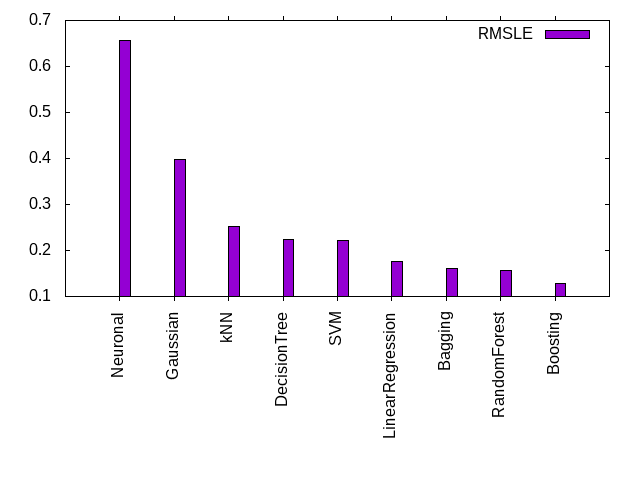
\includegraphics[scale=0.75]{./img/error.png}
	\caption{Test de algoritmos.Error.}
\end{figure}
Se puede observar que los algoritmos que mayor precisión proporcionan en este caso son los multiclasificadores. Por tanto, estudiaremos en profundidad RandomForest y Boosting para mejorar los resultados.
 \section{Herramientas.}
 Otra decisión que debemos de tomar es qué herramientas usar para abordar la resolución del problema. En primer lugar debemos elegir un lenguaje de programación, para tomar esta decisión veremos el rendimiento de algunos de los lenguajes mas usados en data mining(\url{https://www.ibm.com/developerworks/community/blogs/jfp/entry/What_Language_Is_Best_For_Machine_Learning_And_Data_Science?lang=en}). En cada caso usaremos bibliotecas open source(sklearn,weka y librerías de R). Para determinar cual de las 3 es la más conveniente en este caso, realizaré pruebas con los diferentes algoritmos y compararemos el tiempo de ejecución y el uso de memoria. Además, se debe tener en cuenta la facilidad para tratar los datos tanto para su lectura, como para la generación de los archivos con las predicciones. 
 
 Los resultados obtenidos se muestran en las siguientes gráficas:	
 \begin{figure}[!h]
 	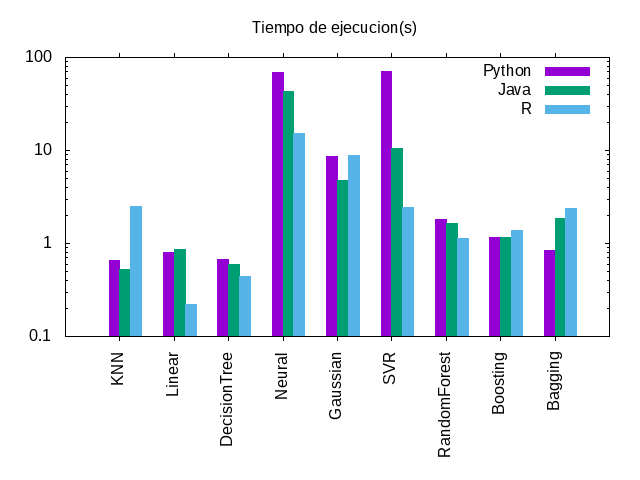
\includegraphics[scale=0.75]{./img/tiempos.png}
 	\caption{Test de algoritmos.Tiempo de ejecución}
 \end{figure}
 \begin{figure}[H]
 	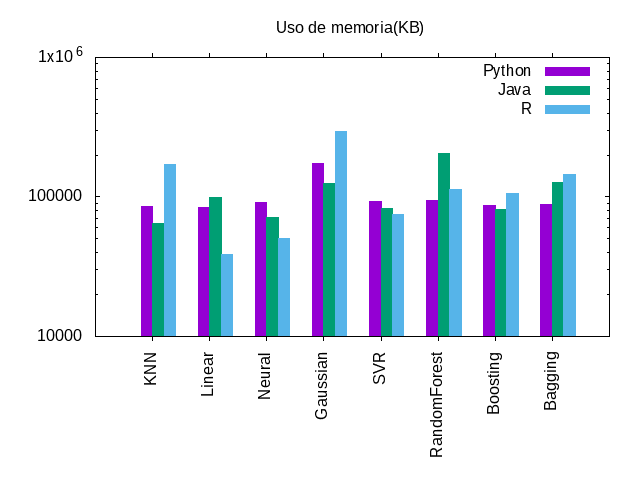
\includegraphics[scale=0.75]{./img/memoria.png}
 	\caption{Test de algoritmos.Memoria usada}
 \end{figure}
 De los resultados se deduce que no existe una alternativa que nos proporcione un rendimiento claramente superior al resto. 
 En conclusión, el lenguaje a usar será Python ya que permite un manejo de los datos flexible y un código legible propio de este lenguaje. Esta decisión se apoya en que en términos de rendimiento no hay una alternativa "mucho mejor". 
\section{Preprocesamiento}
En primer lugar elimino los outliers.Pruebo varios valores de contaminacion y me quedo el optimo.Normalizar datos. Cambiar datos missing por None(se puede entender que NaN quiere decir que no hay?)
%%VERIFICA

%%%%%%%%%%%%%%%%%%%%%%%%%%%%%%%%%%%%%%%%%%%%%%%%%%%%%%%%%%%%%%%%%%%%%%%%%%%%%%%%%%%%%%%%%%
% Segundo curso M'etodos Num'ericos II                                                   %
%                                                                                        %
% Capitulo 2. Derivación e integración numérica.                                         %
%                                                                                        %
% ** NO **  2.1. Breve repaso de interpolación. Fórmulas de Lagrange y Newton.           %
%                                                                                        %
%           2.1. Introducci\'on.                                                         %
%           2.2. Fórmulas de tipo interpolatorio. Orden de exactitud.                    % 
%           2.3. Derivación numérica. Error.                                             %
%           2.4. Fórmulas simples y compuestas de integración numérica. Error.          %
%           2.5. Integración Romberg. Integración adaptativa.                            %
%           2.6. Fórmulas de cuadratura gaussiana.                                       %
%%%%%%%%%%%%%%%%%%%%%%%%%%%%%%%%%%%%%%%%%%%%%%%%%%%%%%%%%%%%%%%%%%%%%%%%%%%%%%%%%%%%%%%%%%


\chapter[Derivaci\'on e integraci\'on num\'erica]
        {Derivaci\'on e integraci\'on \\ num\'erica}

La necesidad de derivar o integrar num\'ericamente una funci\'on $f$ puede justificarse por varios motivos. En el mejor de los casos, puede ocurrir que conozcamos la expresi\'on expl\'{\i}cita de la funci\'on derivada o de la primitiva, pero la expresi\'{o}n puede ser tan complicada que es necesario recurrir a aproximaciones para su evaluaci\'{o}n, que incluso puede provocar errores de igual o mayor magnitud que los cometidos en la propia derivaci\'on o integraci\'on num\'erica. 

Un segundo motivo que justifica la inclusi\'on de este tema podr\'{\i}a ser la dificultad de derivar una funci\'on si \'esta tiene una expresi\'on complicada o dif\'{\i}cil de derivar, o incluso, como ya saben los alumnos, existen funciones que, a\'un siendo integrables, carecen de primitivas expresables en t\'erminos de funciones elementales. 
  
Finalmente, en muchos casos desconocemos la expresi\'on expl\'{\i}cita de la funci\'on que se necesita derivar o integrar, y s\'olo se conocen los valores de la funci\'on en un conjunto finito de puntos $x_0, x_1,\ldots, x_n$.

\section{Introducci\'on}

La derivaci\'on y la integraci\'on num\'erica son problemas muy
similares en su planteamiento. Ambas representan la aproximaci\'on
de un funcional lineal $\mathcal{L}$ definido sobre un espacio de funciones $\mathcal{F}$ 
por una combinaci\'on lineal finita
$\mathcal{L}_n$ de otros funcionales lineales m\'as sim\-ples~$L_i$
$$
  \mathcal{L}_n = \sum_{i=0}^n a_i\,L_i.    
$$
Dada una funci\'on $f\in \mathcal{F}$, una f\'omula de derivaci\'on o integraci\'on num\'erica viene dada por
la expresi\'on
\begin{equation}
\mathcal{L}(f) \approx \mathcal{L}_n(f) = \sum_{i=0}^n a_i\,L_i(f). \label{eq:primera}
\end{equation}
Definiremos el {\it error} de la f\'ormula anterior para la funci\'on $f$ como
$$R(f) = \mathcal{L}(f) - \mathcal{L}_n(f).
$$
As\'{\i}, diremos que la f\'ormula \eqref{eq:primera} es {\it exacta} para una funci\'on $\phi$ si
$$R(\phi) = 0,$$
y diremos que es exacta en un subespacio de funciones $V \subseteq \mathcal{F}$ si es exacta para toda funci\'on de $V$. Si una f\'ormula es exacta en
$V=\Pi_n$ se suele decir que su {\it orden de exactitud} o su {\it grado de exactitud} es $n$.

La forma m\'as simple de una f\'ormula \eqref{eq:primera} es usar datos lagrangianos $L_i(f) = f(x_i)$, con $x_i\neq x_j, i\neq j$, y as\'{\i}
\begin{equation}\label{lagr}
\mathcal{L}(f) \approx \mathcal{L}_n(f)=\sum_{i=0}^n a_i\,f(x_i).
\end{equation}
Si $\mathcal{L}(f) = f^{(k)}(c)$, $k\ge1$, tenemos f\'ormulas de {\it derivaci\'on num\'erica}
\begin{equation}\label{eq:dernum}
  f^{(k)}(c) \approx \mathcal{L}_n(f)=\sum_{i=0}^n a_i\,f(x_i),  
\end{equation}
mientras que si $\displaystyle \mathcal{L}(f)=\int_a^b\!\! f(x)dx$, 
\begin{equation}\label{eq:intnum}
  \int_a^b\!\! f(x)dx \approx \mathcal{L}_n(f)=\sum_{i=0}^n a_i\,f(x_i),  
\end{equation}
obtenemos f\'ormulas de {\it integraci\'on num\'erica}.


\section{Fórmulas de tipo interpolatorio. Exactitud}

El procedimiento m\'as sencillo en este tipo de aproximaci\'on se basa en la
interpolaci\'on. Normalmente el funcional $\mathcal{L}$ presenta dificultades para
aplicarlo a una funci\'on arbitraria de cierto espacio $\mathcal{F}$ de funciones, como
sucede, por ejemplo, al intentar integrar
$f \in {\cal C}[a,b]$, pero por el contrario
es f\'acil de aplicar a las funciones de un subespacio $V$ de 
dimensi\'on finita de $\mathcal{F}$. Entonces el
procedimiento consiste en sustituir $f$ por su funci\'on interpoladora $p(x)$
en $V$ y a continuaci\'on tomar
$$
\mathcal{L}(f) \approx \mathcal{L}_n(f) = \mathcal{L}(p).
$$
En tal caso se dice que la f\'ormula es {\it de tipo interpolatorio}. En este caso, por la linealidad del operador, se verifica
$$R(f) = \mathcal{L}(f) - \mathcal{L}_n(f) = \mathcal{L}(f) - \mathcal{L}(p) = \mathcal{L}(f-p) = \mathcal{L}(E(x)),$$
donde $p$ es la funci\'on interpoladora de $f$, y 
$$E(x) = f(x) - p(x) = f[x_0,\ldots,x_n,x] \prod_{i=0}^n (x-x_i),
$$
es el error de interpolaci\'on. La interpolaci\'on m\'as utilizada es la {\it interpolaci\'on polinomial} en la que $V = \Pi_n$ con datos lagrangianos $L_i(f) = f(x_i),\ i=0, 1, \ldots,n$. En este caso, podemos demostrar el siguiente resultado, que es de gran aplicaci\'on tanto en la construcci\'on de f\'ormulas de
tipo interpolatorio como en el estudio del error de las mismas:

\smallskip
\noindent
{\em
``Son equivalentes:
\begin{enumerate}
\item la f\'ormula \eqref{lagr} es de tipo interpolatorio, 

\item la f\'ormula es exacta en $\Pi_n$, es decir, $R(p) = 0\quad \forall p \in \Pi_n.$

\item los coeficientes o pesos de la f\'ormula se pueden obtener 
$$a_i = \mathcal{L}(\ell_i(x)),\quad i=0, 1, \ldots, n,$$ 
donde $\{\ell_i(x), i=0, 1, \ldots, n\}$ son las funciones b\'asicas de la f\'ormula de interpolaci\'on de Lagrange.''
\end{enumerate}
}
\smallskip

Este resultado proporciona tres formas distintas de construir f\'ormulas de tipo
interpolatorio. La primera consiste en hallar el
polinomio de interpolaci\'on y aplicarle el funcional $\mathcal{L}$, la segunda, llamada el {\it m\'etodo de los coeficientes indeterminados} impone exactitud de la f\'ormula para una base de $V$, y la tercera forma consiste en calcular los coeficientes $a_i$ aplicando el funcional $\mathcal{L}$ a los $\ell_i(x)$ de la base de Lagrange.



\section{Derivaci\'on num\'erica. Error}

Como consecuencia del teorema anterior, si queremos obtener una f\'ormula (\ref{eq:dernum}) de tipo
interpolatorio para aproximar $\mathcal{L}(f)= f^{(k)}(c)$, $k\ge 1$, podemos seguir tres
procedimientos:
\begin{enumerate}
\item hallar el polinomio de interpolaci\'on $p(x)$ de $f(x)$ en los datos dados, y a continuaci\'on aproximar mediante
      $f^{(k)}(c) \approx p^{(k)}(c)$,
      
\item imponer a (\ref{eq:dernum}) exactitud en el espacio $\Pi_n$,
      lo que equivale a resolver el sistema
      $$
      \sum_{i=0}^n \,a_i \,x_i^j= 
      \begin{cases}
         0, & \quad 0 \le j \le k-1,         \\
\frac{\displaystyle{j!}}{\displaystyle{(j-k)!}}\,c^{j-k}, &
        \quad  k \le j \le n,
      \end{cases}
      $$
cuya matriz de coeficientes lleva asociado el determinate de Vandermonde, que es no nulo cuando los nodos $x_i$ son distintos entre s\'{\i},
\item hallar los $\ell_i$ de Lagrange, y tomar $a_i = \ell_i^{(k)}(c).$
\end{enumerate}

Por \'ultimo, existe un procedimiento m\'as para obtener (\ref{eq:dernum})
basado en el desarrollo de Taylor. Para ello supongamos que $f$ es de clase
${\cal C}^{m+1}$ con $m \ge n$, y denotemos por $h_i = x_i - c,\ i=0,\ldots,n$.
Entonces
\begin{eqnarray}
  \lefteqn{f(x_i)  =  f(c+h_i)}            \nonumber         \\*
  & = & f(c) + h_i\,f'(c) +\cdots +\frac{h_i^m}{m!}\,f^{(m)}(c)
              +\frac{h_i^{m+1}}{(m+1)!}\,f^{(m+1)}(\xi_i), \qquad \label{eq:taylor}   
\end{eqnarray}
con $c < \xi_i < c+h_i$, $i=0,1, \ldots,n$. Multiplicando las igualdades (\ref{eq:taylor}) 
por $a_0,\ldots,a_n$
respectivamente, y su\-man\-do, se ob\-tie\-ne
\begin{eqnarray*}
 \sum_{i=0}^n a_i f(x_i) &=& f(c)\sum_{i=0}^n a_i
                                  + f'(c) \sum_{i=0}^n a_i h_i +\cdots \\*
 && \qquad + \frac{f^{(m)}(c)}{m!} \sum_{i=0}^n a_i h_i^m
        + \frac{1}{(m+1)!}\sum_{i=0}^n a_i \,h_i^{m+1} \,f^{(m+1)}(\xi_i).
\end{eqnarray*}
Si imponemos las condiciones
$$\sum_{i=0}^n \, a_i\, h_i^j = k!\,\delta_{jk},\quad j=0,1,\ldots,n,
$$
obtenemos un sistema de ecuaciones que hace que la f\'ormula (\ref{eq:dernum}) sea exacta en $\Pi_n$. 
Adem\'as, este sistema es compatible determinado, ya que los $h_i$ son todos
distintos al serlo los $x_i$, y la matriz de coeficientes
lleva asociado de nuevo el determinante de Vandermonde. 

Cuando los puntos $x_i$ son equidistantes, la expresi\'on de las f\'ormulas es
m\'as simple pues en tal caso pueden usarse las f\'ormulas de interpolaci\'on de Newton progresiva o regresiva para obtener $p(x)$ en funci\'on de las diferencias finitas.

\bigskip

Deduciremos las f\'ormulas habituales de derivaci\'on num\'erica utilizando alternativamente todos los m\'etodos descritos anteriormente. Clasificaremos las f\'ormulas seg\'un el n\'umero de datos lagrangianos utilizados: uno, dos, tres nodos, y su posici\'on relativa atendiendo al punto en el cual se desea aproximar la derivada.

\subsection*{Error en derivaci\'on num\'erica}

En este caso, el error se calcular\'a en la forma
$$
R(f) = \mathcal{L}(E(x))= \left.\frac{d^k}{dx^k}E(x)\right|_{x=c} =
    \left.\frac{d^k}{dx^k}\Big(f[x_0,\ldots,x_n,x]\, \pi(x)\Big)\right|_{x=c}
$$
donde $\displaystyle \pi(x) = \prod_{i=0}^n (x-x_i)$.
Si $k=1$ y $f$ es derivable, se obtiene
$$
  R(f) = \left.\left(f[x_0,\ldots,x_n,x,x]\,\pi(x) + f[x_0,\ldots,x_n,x]\,\pi'(x)\right)\right|_{x=c}
$$
y si $f$ es de clase ${\cal C}^{n+2}$, podemos escribir
$$
  R(f) = \frac{f^{(n+2)}(\xi)}{(n+2)!}\pi(c) + \frac{f^{(n+1)}(\eta)}{(n+1)!} \pi'(c),
$$
donde $\xi, \eta$ son puntos intermedios, de tal forma que si $c=x_j$ para alg\'un $j$, entonces $\pi(c)=0$, y
$$
  R(f) = \frac{f^{(n+1)}(\eta)}{(n+1)!}\,\pi'(c)
       = \frac{f^{(n+1)}(\eta)}{(n+1)!}\prod_{\substack{ i=0 \\ i \ne j}}^n
         (c-x_i).
$$
De forma an\'aloga, si $f$ es de clase ${\cal C}^{n+k+1}$, la expresi\'on del
error de la derivada $k$--\'esima viene dada por la expresi\'on
$$
  R(f) = \sum_{i=0}^k \frac{k!}{(k-i)!(n+i+1)!}f^{(n+i+1)}(\eta_i)\pi^{(k-i)}(c)
$$
donde los $\eta_i$ pertenecen a cualquier intervalo que contenga a
$x_0,\ldots,x_n,$ y al punto~$c$.

Se puede dar una cota para $R(f)$ si se conocen cotas para
cada una de las derivadas de $f$ que aparecen en la expresi\'on de $R(f)$. Una
forma de rebajar la cota del error es disminuir el n\'umero de sumandos. Ya hemos visto que si $\pi(c) = 0$ se anula un sumando de la expresi\'on del error para cualquier derivada. 

Un caso particularmente sencillo es cuando se usan {\it f\'ormulas centrales}, que son f\'ormulas
 de tipo interpolatorio polinomial que aproximan la derivada en un punto $c= x_0$, usando
como conjunto de nodos uno de los siguientes
$$
  \big\{x_{-r},\ldots,x_{-1},x_1,\ldots,x_r\big\},\quad
  \big\{x_{-r},\ldots,x_{-1},x_0,x_1,\ldots,x_r\big\},
$$
donde los $x_i$ son equidistantes. Utilizando diferencias centrales, se demuestra de forma sencilla 
que si se aproxima la derivada
primera con ambos conjuntos, se obtiene el mismo orden de convergencia. 
Sin embargo, hay ocasiones en las que no pueden usarse f\'ormulas
centrales, como por ejemplo, si se desea estimar la derivada en uno de los extremos del 
intervalo.

\bigskip

Un problema esencial de la derivaci\'on num\'erica es el mal
condicionamiento de las f\'ormulas. Por una parte, de la expresi\'on expl\'{\i}cita del
error de las f\'ormulas observamos que te\'oricamente converge
hacia cero cuando $h$ tiende a cero. Sin embargo, puesto que la
expresi\'on de la f\'ormula contiene una potencia de $h$ en el denominador,
los errores de redondeo crecen indefinidamente cuando $h$ tiende a cero.


\section{Integración numérica. Error}

Abordaremos en esta secci\'on el c\'alculo de la integral definida de una funci\'on real mediante la expresi\'on 
\begin{equation}\label{eq:integral}
  I(f) = \int_a^b\!\! f(x) dx \approx  I_n(f) = \sum_{i=0}^n a_i\, f(x_i).
\end{equation}
Una f\'ormula del tipo anterior se denomina f\'ormula de {\it cuadratura num\'erica\/} o de {\it 
integraci\'on num\'erica}. Las f\'ormulas b\'asicas que se utilizan en la pr\'actica son las de tipo interpolatorio o composici\'on de \'estas. 

\subsection{F\'ormulas simples}
Las f\'ormulas sencillas de integraci\'on num\'erica con uno, dos, tres nodos, rect\'{a}ngulo, punto medio, trapecio y Simpson, se
deducir\'an utilizando la equivalencia entre el car\'acter interpolatorio y la exactitud:
hallando $p(x)$, el polinomio de interpolaci\'{o}n en $x_0, x_1, \ldots, x_n$, y aproximando mediante
      $$\int_a^b\!\! f(x) dx \approx \int_a^b\!\! p(x) dx,$$
imponiendo exactitud en el espacio $\Pi_n$, lo que equivale a resolver el siguiente sistema:
$$\sum_{i=0}^n \, a_i \, x_i^k  =  \frac{1}{k+1}\,(b^{k+1}-a^{k+1}), \quad
                           0 \le k \le n,
$$
o hallando los polinomios b\'asicos $\ell_i(x)$ de Lagrange, y tomando
 $$a_i
=\int_a^b\!\! \ell_i(x) dx.$$

Como ya hemos visto, el error asociado a las f\'ormulas de integraci\'on num\'erica de tipo interpolatorio es
$$
  R(f) = \int_a^b\!\! E(x) dx = \int_a^b\!\! f[x_0,\ldots,x_n,x]\, \pi(x) dx, 
$$
donde $\pi(x) = \prod_{i=0}^n (x-x_i)$. Si el polinomio $\pi(x)$ no cambia de signo en
$[a,b]$ y $f'$ es continua, aplicando el teorema del valor
medio para el c\'alculo integral, se tiene
$$
  R(f) = f[x_0,\ldots,x_n,\xi] \int_a^b\!\! \pi(x)dx,\quad
  \hbox{con}\quad \xi \in (a,b),
$$
y si adem\'as $f \in {\cal C}^{n+1}[a,b]$, 
$$
  R(f) = \frac{f^{(n+1)}(\eta)}{(n+1)!} \int_a^b\!\! \pi(x) dx.
$$
Estas herramientas nos servir\'an para calcular el error en cada una de las f\'ormulas deducidas m\'as arriba.
De este modo, aunque las f\'ormulas del rect\'angulo derecha e izquierda y la del punto medio tienen s\'olo 
un dato, y son exactas en $\Pi_0$, la f\'ormula del punto medio posee {\it m\'as exactitud de la esperada}, 
al igual que la f\'ormula de Simpson, que, aun teniendo tres datos, es exacta en $\Pi_3$.


\subsection*{F\'ormulas de Newton--Cotes}

Las {\it f\'ormulas de
Newton--Cotes\/} utilizan como nodos puntos equidistantes del intervalo $[a,b]$.
Concretamente, si $n$ es un n\'umero natural, se define la partici\'on 
$$x_i = a + i\, h,\quad i=0, 1, \ldots, n,$$
donde $h = (b-a)/n$.

Pueden ser {\it cerradas\/}, que son las que tienen por nodos $x_0,x_1,\ldots,x_n$, o {\it abiertas\/}
que tienen como nodos $x_1,\ldots,x_{n-1}$.

Estas f\'ormulas se pueden obtener siguiendo cualquiera de los procedimientos descritos anteriormente en las
f\'ormulas de tipo interpolatorio. 

Entre las f\'ormulas de Newton--Cotes cerradas m\'as simples
se encuentran la del {\it trapecio\/}, con $n=1$ (dos puntos), y la de {\it Simpson} para $n=2$ (tres puntos), muy utilizadas
en la pr\'actica en sus formas compuestas. Para $n=3$, deduciremos la f\'ormula de los $3/8$ de Newton as\'{\i} como su error.

La f\'ormula de Newton--Cotes abierta m\'as sencilla es la del {\it del punto medio\/}, $n=2$, obtenida anteriomente. Tambi\'en deduciremos la f\'ormula abierta para $n=3$ y su error.

\bigskip

Las f\'ormulas de Newton--Cotes no son estables y no garantizan la convergencia. Como prob\'o Runge con su famoso ejemplo, los polinomios de interpolaci\'on en nodos equidistantes no tienen porqu\'e converger hacia la funci\'on. Este mismo ejemplo servir\'a para mostrar este inconveniente de las f\'ormulas de Newton--Cotes. 


\subsection{F\'ormulas compuestas}

Las expresiones expl\'{\i}citas del error para cada una de las f\'ormulas {\it simples} deducidas anteriomente nos hace ver que no es posible conseguir f\'ormulas que hagan converger el error hacia cero. Una alternativa ser\'{\i}a aumentar
el orden de convergencia pero para ello es necesario utilizar un n\'umero de nodos cada vez m\'as
elevado y, a\'un as\'{\i}, no tenemos garantizada la convergencia. Una f\'ormula que utilice muchos nodos tiene, adem\'as, el inconveniente de
que el c\'alculo de los nodos y de los coeficientes puede ser muy costoso. Una forma
de evitar estas dificultades es utilizar {\it f\'ormulas compuestas}.

Una f\'ormula compuesta se obtiene al aplicar alguna de las f\'ormulas {\it simples}
obtenidas anteriormente a una par\-ti\-ci\'on del intervalo
$[a,b]$. En efecto, sea $N\ge 1$ un n\'umero natural fijo, definimos $h=(b-a)/N$, y los subintervalos
$$[a_i,a_{i+1}], \qquad i=0, 1, \ldots, N-1,$$
donde $a_i = a + i\,h, \, 0\le i \le N$. De este modo, 
$$I(f) = \int_a^b f(x)\, dx = \sum_{i=0}^{N-1}\int_{a_i}^{a_{i+1}} f(x) \,dx,$$
y el error se obtendr\'a como suma de los errores cometidos en cada uno de los 
subintervalos
$$R(f) = \sum_{i=0}^{N-1} R_i(f),$$
donde $R_i(f)$ denota el error cometido en el subintervalo $[a_i,a_{i+1}]$.

As\'\i , por ejemplo, deduciremos la {\it f\'ormula del trapecio compuesta\/} que es
$$
  \int_a^b\!\! f(x)\,dx \approx
  \frac{h}{2}\left[f(a) + 2\!\!\sum_{i=1}^{N-1} f(a_i) + f(b) \right],
$$
y el error cometido, supuesta $f$ de clase ${\cal C}^2$, es
$$
  R(f) = - \frac{b-a}{12} \, h^2 \, f''(\xi),\qquad a<\xi<b.
$$
An\'alogamente, la {\it f\'ormula de Simpson compuesta\/} viene dada por
$$
  \int_a^b\!\! f(x)dx \approx
  \frac{h}{3}\left[f(a) + f(b) + 2\!\sum_{i=1}^{N-1} f(a_i)
              + 4\!\sum_{i=0}^{N-1} f(a_{i} +h/2) \right],
$$
y el error cometido, supuesta $f$ de clase ${\cal C}^4$,
es
$$
  R(f) =\frac{b-a}{2880}\,h^4\,f^{(4)}(\xi),\quad a<\xi<b.
$$
Demostraremos que si se utiliza una f\'ormula de Newton--Cotes compuesta que en
cada subintervalo use $n\ge1$ nodos, el error viene dado por la expresi\'on
$$
R(f)=\left\{\begin{array}{ll}
                  \displaystyle
                  \frac{b-a}{n!}\,\frac{M_n}{n^{n+1}}\,h^n\,f^{(n)}(\xi),
                                                 & \quad a<\xi<b\hbox{,  n par,} \\*
                                 &  \\*
                  \displaystyle
                  \frac{b-a}{(n+1)!}\,\frac{K_n}{n^{n+2}}\,h^{n+1}\,f^{(n+1)}(\xi),
                                                 & \quad a<\xi<b\hbox{,  n impar,}
             \end{array}
       \right.
$$
donde $M_n$ y $K_n$ son constantes.
Obviamente, el error $R(f)$ en las f\'ormulas compuestas asociadas a las f\'ormulas de Newton--Cotes tiende hacia a cero cuando $h \rightarrow 0$.



\section{Integración Romberg}

La integraci\'on Romberg es un proceso de extrapolaci\'on que puede aplicarse a la f\'ormula del trapecio compuesta y que permite obtener mejores aproximaciones a la integral definida de una funci\'on dada. En esta secci\'on denotamos por
$$I(f) =  \int_a^b\!\! f(x)dx,$$
la integral exacta de la funci\'on $f$, y 
$$T(f,h) = \frac{h}{2}\left[f(a) + 2\!\!\sum_{i=1}^{N-1} f(a+ih) + f(b) \right],$$
la f\'ormula del trapecio compuesta, donde $N\ge 1$, $h = (b-a)/N.$

La integraci\'on Romberg se basa en la
\begin{thm}[F\'ormula de Euler--McLaurin]
Si para alg\'un $n\ge 1$, $f \in \mathcal{C}^{2n+1}[a,b]$ entonces 
$$T(f,h) = I(f) + g_1\,h^2 + g_2\,h^4 + \ldots + g_n\,h^{2n} + \mathcal{O}(h^{2n+1}), \quad h\to 0, $$
donde los coeficientes tienen la expresi\'on expl\'{\i}cita
$$g_k = \frac{B_{2k}}{(2k)!}\left[f^{(2k-1)}(b) - f^{(2k-1)}(a)\right], \quad k=1, 2, \ldots, n,$$
y $B_{2k}$ denota el n\'umero de Bernouilli.
\end{thm}
A partir de la f\'ormula de Euler--McLaurin conocemos el desarrollo asint\'otico del error para la f\'ormula del trapecio compuesta, lo que permite mejorar este resultado tomando
\begin{eqnarray*} 
&~& T(f,h) = I(f) + g_1\,h^2 + g_2\,h^4 + g_3\,h^6 + \ldots \\
&~& T(f,h/2) = I(f) + g_1\,(h/2)^2 + g_2\,(h/2)^4 + g_3\,(h/2)^6+ \ldots
\end{eqnarray*}
y eliminando el t\'ermino en $g_1$, esto es, 
$$\frac{4\,T(f,h/2) - T(f,h)}{3} = I(f) + \tilde{g_2}\,h^4 + \tilde{g_3}\,h^6+ \ldots,$$
con lo que obtenemos una aproximaci\'on de la integral $I(f)$ con un error del orden de $\mathcal{O}(h^4)$. Podemos repetir de nuevo este proceso para eliminar el t\'ermino en $h^4$, y as\'{\i} sucesivamente. Para $m=0, 1, \ldots$, y $1\le k\le m$, definimos
\begin{eqnarray*}
R(m,0) &:=& T\big(f,\frac{b-a}{2^m}\big),\\
R(m,k) &:=& \frac{4^k\,R(m,k-1) - R(m-1,k-1)}{4^k - 1}\\
               &=& R(m,k-1) + \frac{R(m,k-1) - R(m-1,k-1)}{4^k - 1}.
\end{eqnarray*}
Podemos disponer los c\'alculos en una sencilla tabla de valores
$$
\begin{array}{ccccccc}
R(0,0) &~                &        &~                &        &~                &        \\
~      & \searrow        &        &                 &        &                 &        \\
R(1,0) & \longrightarrow & R(1,1) &                 &        &                 &        \\
~      & \searrow        &        & \searrow        &        &                 &        \\
R(2,0) & \longrightarrow & R(2,1) & \longrightarrow & R(2,2) &                 &        \\
~      & \searrow        &        & \searrow        &        & \searrow        &        \\
R(3,0) & \longrightarrow & R(3,1) & \longrightarrow & R(3,2) & \longrightarrow & R(3,3) \\
~      &                 &        &                 &        &                 &        \\
\vdots &                 & \vdots &                 & \vdots &                 & \vdots
\end{array}
$$
El siguiente resultado asegura la convergencia de la integraci\'on Romberg:
\begin{thm}
Sea $f\in \mathcal{C}^{2n+1}[a,b]$ para alg\'un $n\ge 1$. Sea $m\ge 0$, $1\le k\le n$
$$R(m,k) = I(f) + \mathcal{O}(h^{2k}), \quad h=\frac{b-a}{2^m} \to 0.$$
\end{thm}
\noindent
En particular, para todo $k\le n$, se cumple que
$$\lim_{m\to \infty} R(m,k) = \int_a^b f(x) \,dx.$$


\section{F\'ormulas de cuadratura gaussiana}

Ya se ha visto en las secciones anteriores que las f\'ormulas de tipo interpolatorio con $n+1$ nodos tienen, al menos, grado de exactitud $n$, aunque algunas f\'ormulas, por ejemplo, las de Newton--Cotes con n\'umero impar de nodos, superan este grado de exactitud. Nos planteamos en esta secci\'on si eligiendo adecuadamente los nodos se puede obtenerse m\'as exactitud, e incluso cu\'al es el m\'aximo grado de exactitud que se puede obtener para un 
n\'umero de nodos fijo. En este sentido, demostraremos el siguiente 

\begin{thm}
Sea $\omega(x)$ una funci\'on peso. Consideremos la f\'ormula de integraci\'on num\'erica
\begin{equation} \label{formula}
  I(f) = \int_a^b\!\! f(x)\,\omega(x)\,dx \approx a_0 \,f(x_0) + a_1\,f(x_1) + \ldots + a_n \,f(x_n),
\end{equation}
y definamos  $\pi(x)=(x-x_0)\,(x-x_1)\ldots(x-x_n)$. Entonces
\begin{itemize}
\item[\bf (i)] la f\'ormula \eqref{formula} tiene orden de exactitud $n+q$, $q\ge 1$, si y s\'olo si es de tipo interpolatorio, y los nodos $x_j$ cumplen
      $$
       \int_a^b\!\! \pi(x)\,x^k\,\omega(x)\,dx = 0,\quad k=0,1,\ldots,q-1.
      $$
\item[\bf (ii)] \eqref{formula} no puede tener orden de exactitud mayor o igual a $2n+2$.
\item[\bf (iii)] Existen $n+1$ puntos distintos $x_j \in (a,b)$, $j=0,\ldots,n$, tales que \eqref{formula} tiene orden de exactitud $2n+1$.
\end{itemize}
\end{thm}
A las f\'ormulas de integraci\'on num\'erica que tienen orden de exactitud m\'aximo se las denomina
{\it f\'ormulas de cuadratura gaussianas} o {\it f\'ormulas de Gauss}, mientras que a las f\'ormulas de tipo interpolatorio que tienen orden de exactitud $n+q$ con $2\le q<n$ se les llama de {\it tipo Gauss}.

Utilizando el resultado anterior, si \eqref{formula} es una f\'ormula de Gauss, entonces tiene por nodos
las ra\'\i ces del polinomio ortogonal $P_{n+1}(x)$ asociado respecto al producto
escalar
$$
 \langle f,g \rangle = \int_a^b\!\! f(x)\,g(x)\,\omega(x)\,dx.
$$
Algunas f\'ormulas gaussianas reciben nombres espec\'\i ficos que corresponden
con funciones peso concretas, bien conocidas en la literatura. Por ejemplo, si $[a,b]=[-1,1]$, podemos citar
\begin{itemize}
\item si $\omega(x) = 1$, se denomina {\it f\'ormula de Gauss--Legendre},
\item si $\omega(x) = (1-x^2)^{-1/2}$, se denomina {\it de Gauss--Chebyshev}, 
\item en general, si $\omega(x) = (1-x)^\alpha(1+x)^\beta$, $\alpha, \beta >-1$, se llama {\it de Gauss--Jacobi}.
\end{itemize}
Un resultado fundamental que muestra el error de las f\'ormulas
gaus\-sia\-nas es el si\-guien\-te:

\smallskip
\noindent
{\em
``Si $f$ es de clase ${\cal C}^{n+2}$ en $[a,b]$ y \eqref{formula} es una
f\'ormula gaussiana, entonces el error correspondiente puede expresarse como
$$
  R(f) = \frac{f^{(n+2)}(\xi)}{(n+2)!} \,\int_a^b\!\! \pi^2(x)\,\omega(x)dx
  \hbox{''.}
$$
}
\smallskip

Las f\'ormulas gaussianas poseen propiedades muy interesantes: los
coeficientes de las f\'ormulas $a_i$ son todos positivos, lo que implica la estabilidad de 
estas f\'ormulas. Adem\'as, se da la convergencia de las f\'ormulas
de cuadratura gaussianas para toda funci\'on continua en $[a,b]$ al valor de la integral cuando
$n \rightarrow \infty$.

Frente a propiedades de estabilidad, convergencia, y orden elevado de
exactitud, las f\'or\-mu\-las gaus\-sia\-nas tambi\'en pre\-sen\-tan in\-con\-ve\-nien\-tes. 
Para deducir las f\'ormulas gaussianas es necesario hallar los nodos, y para ello hay que obtener el polinomio ortogonal, calcular sus ra\'\i ces, que suelen ser n\'umeros irracionales, y despu\'es hay que calcular los coeficientes, lo que obliga a cometer errores de redondeo
desde la misma f\'ormula. Por otro lado, si se tiene una f\'ormula de Gauss
con $n$ nodos y se desea obtener una con $n+1$ nodos, es necesario rehacer todos
los c\'alculos de nuevo, dado que no existe una ley de recurrencia para obtener
los ceros de los polinomios ortogonales. As\'\i\  pues, este tipo de
f\'ormulas no son pr\'acticas para esquemas autom\'aticos.

\section{Pr\'actica de laboratorio}

En las {\it pr\'{a}cticas de laboratorio} propondremos a los alumnos la deducci\'on y aplicaci\'on de algoritmos de {\it integración adaptativa} basados en diversas f\'ormulas de integraci\'on num\'erica. 

Estudiaremos los llamados {\it esquemas autom\'aticos}, recientemente desarrollados, que son programas que,
partiendo de los l\'\i mites de integraci\'on, el integrando y el error
admisible, calculan una aproximaci\'on de la integral.  Tambi\'en es interesante estudiar las rutinas para integraci\'{o}n num\'erica
basadas en cuadraturas gaussianas \textit{QUADPACK}

\url{http://www.netlib.org/quadpack/}

Escritas originalmente en FORTRAN, han sido implementadas también en
diferentes lenguajes de alto nivel (C, Python, \ldots).

Alternativamente, podr\'{\i}a ser
interesante considerar las rutinas para 
integraci\'on num\'erica de \textit{ALGLIB}

\url{http://www.alglib.net}

Existen versiones de estas rutinas en diferentes
lenguajes de alto nivel (C++, C\#, Pascal, VBA).


\section{Comentarios bibliogr\'aficos}

Las f\'{o}rmulas de derivaci\'{o}n num\'erica de tipo interpolatorio, o las basadas en desarrollos
de Taylor junto con el correspondiente an\'{a}lisis del
error  se estudian en profundidad en Atkinson \cite{At3}, Gautschi
\cite{Ga13}, Stewart \cite{stewart} y Ralston \cite{Ra}. 

La cuadratura o integraci\'on num\'erica es una de las materias estudiada desde m\'as antiguo, y 
es b\'asica en el An\'alisis Num\'erico, lo que hace que sea tratada en muchas obras de la
bibliograf\'\i a de este Proyecto. 

Una referencia fundamental para integraci\'on num\'erica es el
texto de W. Gautschi \cite{Ga13}, en el que podemos encontrar
un buen tratamiento de las f\'ormulas de cuadratura simples, de
las f\'ormulas gaussianas, de los algoritmos de c\'alculo de 
los coeficientes y los nodos, y de la integraci\'on Romberg. Otros
textos complementarios son los de Ralston 
\cite{Ra}, Kincaid y Cheney \cite{KCh},
Burden y Faires \cite{BF}, Stewart \cite{stewart} o Stoer
y Bulirsch \cite{SB}.

%\begin{thebibliography}{100}
\addcontentsline{toc}{chapter}{Bibliograf\'{\i}a}


\bibitem{At3} 
K.~E. Atkinson,
\newblock {\it An introduction to Numerical Analysis}, 2nd ed.,
\newblock Wiley, New York, 1989.

\bibitem{BF} 
L.~R. Burden, D.~J. Faires,
\newblock {\it An\'alisis Num\'erico}, S\'eptima Edici\'on,
\newblock Thomson Learning, M\'exico, 2003.


\bibitem{Ga13} 
W. Gautschi,
\newblock{\it Numerical analysis}, 2nd ed.,
\newblock Birkh\"auser--Science Springer, New York Dordrecht Heidelberg London 2012.

\bibitem{KCh}
D. Kincaid, W. Cheney,
\newblock {\it  An\'alisis Num\'erico. Las matem\'aticas del c\'alculo
cient\'{\i}fico},
\newblock Addison--Wesley Iberoamericana, Wilmington, 1994.

\bibitem{Ra} 
A. Ralston,
\newblock {\it Introducci\'on al An\'alisis Num\'erico},
\newblock Limusa--Wiley, M\'exico, 1970.

\bibitem{stewart} 
G. W. Stewart,
\newblock {\it Afternotes on Numerical Analysis},
\newblock SIAM, Philadelphia, 1996.

\bibitem{SB} 
J. Stoer, R. Burlirsch,
\newblock {\it Introduction to numerical analysis}, 3rd. ed.,
\newblock Springer, New York, 2002.

\end{thebibliography}




\end{document}

